\chapter{椭圆曲线的基本理论}\label{ch:2}

\section{椭圆曲线的定义}\label{sec:2.1}

\begin{definition} \label{thm:2.1.1} 
域 $k$ 上的椭圆曲线 (elliptic curve) 可以按口味被定义为:
\begin{enumerate}[label=\textup{(\alph*)}]
\item $k$ 上带有点 $O\in E(k)$ 的次数为 $3$ 的非奇异射影平面曲线 $E$;
\item 同 (a), 但要求 $O$ 为拐点 (point of inflection);
\item $k$ 上形如
\begin{equation} \label{eq:9}
Y^2Z + a_1XYZ + a_3YZ^2 = X^3 + a_2X^2Z + a_4XZ^2 + a_6Z^3
\tag{9}
\end{equation}
的非奇异射影平面曲线;
\item $k$ 上亏格为 $1$、带有点 $O\in E(k)$ 的非奇异完备曲线 $E$.
\end{enumerate}
\end{definition}

各定义之间的蕴含关系如下.

(a)$\implies$(d). 设 $E$ 如 (a). 则由公式~\eqref{eq:6}, $E$ 的亏格为 $1$.

(d)$\implies$(c). 设 $(E,O)$ 如 (d). 我们将在第~\pageref{subsec:genus1-embedding}~页看到 Riemann--Roch 定理蕴含 $k$-向量空间 $L(3O)$ 有基 $1, x, y$, 使得映射
\[
P\mapsto(x(P):y(P):1)\colon E\setminus\{O\}\to\mathbb{P}^2
\]
定义 $E$ 到曲线 \eqref{eq:9} 的同构, 把 $O$ 送到 $(0:1:0)$.

(b)$\iff$(c). 设 $(E,O)$ 如 (b). 我们将在命题 \ref{thm:2.1.2} 中证明变量的线性替换把 $E$ 化为形式 (c), 并把 $O$ 送到点 $(0:1:0)$. 反之, 设 $E$ 如 (c), 则 $O = (0:1:0)\in E(k)$ 且是拐点 (I\ref{thm:1.1.20}).

(b)$\implies$(a). 显然.

合并这些陈述, 我们看到如 (a) 的曲线 $E$ 可嵌入 $\mathbb{P}^2$, 使 $O$ 成为拐点. 我们也将给出这一点的直接证明 (第~\pageref{subsec:genus1-embedding}~页).

为明确起见, 我们采用 (d) 作为椭圆曲线的定义.

\subsection*{把三次方程化为标准形式}

\begin{proposition} \label{thm:2.1.2} 
设 $C$ 为 $k$ 上的非奇异三次射影平面曲线, $O\in C(k)$ 为拐点.
\begin{enumerate}[label=\textup{(\alph*)}]
\item 经过一次以 $k$ 中系数实施的线性可逆变量替换后, 点 $O$ 的坐标变为 $(0:1:0)$, 且 $C$ 在 $O$ 处的切线为直线 $Z = 0$.
\item 若 $O = (0:1:0)$ 且 $C$ 在 $O$ 处的切线为 $Z = 0$, 则 $C$ 的方程具有形式~\eqref{eq:9}.
\end{enumerate}
\end{proposition}

\begin{proof}
先证 (a). 设 $(a:b:c)\in\mathbb{P}^2(k)$, 且假设 $b\neq 0$. 正则映射
\[
(x:y:z)\mapsto(bx-ay:by:bz-cy)\colon\mathbb{P}^2\to\mathbb{P}^2
\]
把 $(a:b:c)$ 送到 $(0:b^2:0) = (0:1:0)$, 且是同构 (它有类似形式的逆). 若 $b = 0$ 而 $c\neq 0$, 例如, 则先交换 $y$ 与 $z$ 坐标. 因此可设 $O = (0:1:0)$.

设
\[
L\colon aX + bY + cZ = 0, \qquad a,b,c\in k,
\]
为 $(0:1:0)$ 处的切线. 设 $A = (a_{ij})$ 为前两列正交于 $(a,b,c)$ 的任意可逆 $3\times 3$ 矩阵, 并用下式定义变量替换:
\[
A\begin{pmatrix}X'\\ Y'\\ Z'\end{pmatrix} = \begin{pmatrix}X\\ Y\\ Z\end{pmatrix}.
\]
关于变量 $X', Y', Z'$, 直线 $L$ 的方程变为
\[
0 = (a,b,c)\begin{pmatrix}X\\ Y\\ Z\end{pmatrix} = (a,b,c)A\begin{pmatrix}X'\\ Y'\\ Z'\end{pmatrix} = (0,0,d)\begin{pmatrix}X'\\ Y'\\ Z'\end{pmatrix} = dZ'.
\]
且 $d\neq 0$, 故可把直线方程取为 $Z' = 0$. (a) 的证明完毕.

现在假设 $C$ 与 $O$ 满足 (b) 的条件. 一般三次型为
\[
c_1X^3 + c_2X^2Y + c_3X^2Z + c_4XY^2 + c_5XYZ + c_6XZ^2 + c_7Y^3 + c_8Y^2Z + c_9YZ^2 + c_{10}Z^3.
\]
设 $F(X,Y,Z)$ 为定义 $C$ 的多项式. 因 $C$ 非奇异, $F$ 几何不可约 (I\ref{thm:1.1.21}).

因 $O = (0:1:0)\in C(k)$, $c_7 = 0$.

回忆 $U_1 = \{(x:y:z) \mid y\neq 0\}$, 且把 $U_1$ 等同于 $\mathbb{A}^2$ 由 $(x:1:z)\leftrightarrow(x,z)$. 且 $C\cap U_1$ 是由 $F(X,1,Z)$ 定义的仿射曲线:
\[
c_1X^3 + c_2X^2 + c_3X^2Z + c_4X + c_5XZ + c_6XZ^2 + c_8Z + c_9Z^2 + c_{10}Z^3.
\]
$(0:1:0)\leftrightarrow(0,0)$ 处的切线是直线 $c_4X + c_8Z = 0$. 因它等于直线 $Z = 0$, $c_4 = 0$. 又因 $C$ 非奇异, $c_8\neq 0$.

设 $L$ 为直线 $Z = 0$. 相交数
\[
I(O, L\cap C) = I(Z, F(X,1,Z)) \overset{\text{\ref{thm:2.1.8}d}}{=} I(Z, c_1X^3 + c_2X^2).
\]
因 $O$ 是拐点, $I(O, L\cap C)\ge 3$, 故 $c_2 = 0$.

合并加框的结论, 我们发现三次型化为
\[
c_1X^3 + c_3X^2Z + c_5XYZ + c_6XZ^2 + c_8Y^2Z + c_9YZ^2 + c_{10}Z^3, \qquad c_8\neq 0.
\]
且 $c_1\neq 0$, 否则多项式被 $Z$ 整除. 除以 $c_1$ 并把 $Z$ 换成 $-c_1Z/c_8$ 后, 得到形如 \eqref{eq:9} 的方程.
\end{proof}

\subsection*{带有理点的亏格 $1$ 曲线的射影嵌入}\label{subsec:genus1-embedding}
设 $E$ 为域 $k$ 上亏格 $1$ 的完备非奇异曲线, $O\in E(k)$. 由 Riemann--Roch 定理 (I\ref{thm:1.4.13}), $E$ 上除在 $O$ 处有至多 $m\ge 1$ 阶极点外无其他极点的有理函数, 构成 $k$ 上的 $m$ 维向量空间, 即对 $m\ge 1$, $L(m[O])$ 的维数为 $m$. 常数函数属于 $L([O])$, 故 $\{1\}$ 是 $L([O])$ 的基. 选取 $x$ 使 $\{1,x\}$ 为 $L(2[O])$ 的基, 再取 $y$ 使 $\{1,x,y\}$ 为 $L(3[O])$ 的基. 集合 $\{1,x,y,x^2\}$ 线性无关, 因而是 $L(4[O])$ 的基, 否则 $x^2$ 将是 $1,x,y$ 的线性组合, 不可能在 $O$ 处有四重极点. 类似地, $\{1,x,y,x^2,xy\}$ 是 $L(5[O])$ 的基.

$L(6[O])$ 的子集 $\{1,x,y,x^2,xy,x^3,y^2\}$ 含 $7$ 个元素, 故必线性相关:
\[
a_0y^2 + a_1xy + a_3y = a_0'x^3 + a_2x^2 + a_4x + a_6, \qquad a_i\in k,
\]
作为 $E\setminus\{O\}$ 上的正则函数. $a_0$ 与 $a_0'$ 都非零, 因为去掉 $x^3$ 或 $y^2$ 后集合都线性无关; 把 $y$ 换成 $a_0y/a_0'$, 把 $x$ 换成 $a_0x/a_0'$, 并乘以 $a_0'^2/a_0^3$ 后, 可设两者都等于 $1$. 映射
\[
P\mapsto(x(P), y(P))
\]
把 $E\setminus\{O\}$ 送到仿射平面曲线
\[
C\colon Y^2 + a_1XY + a_3Y = X^3 + a_2X^2 + a_4X + a_6.
\]
函数 $x$ 在 $O$ 处有二重极点且无其他极点, 故它恰有两个零点. 类似地, 对每个 $c\in k$, $x + c$ 有两个零点 (计入重数), 故复合映射
\[
E\setminus\{O\}\to C\to\mathbb{A}^1, \qquad
P\mapsto(x(P), y(P))\mapsto x(P)
\]
的次数为 $2$ (见I~\ref{thm:1.4.24}, \ref{thm:1.4.26}). 类似地, 复合映射
\[
E\setminus\{O\}\to C\to\mathbb{A}^1, \qquad
P\mapsto(x(P), y(P))\mapsto y(P)
\]
的次数为 $3$. 因此 $P\mapsto(x(P), y(P))\colon E\setminus\{O\}\to C$ 的次数整除 $2$ 与 $3$, 故等于 $1$, 即 $k(C)\cong k(E)$. 若 $C$ 奇异, 则其相伴的非奇异曲线 $E$ 亏格为 $0$, 与假设矛盾. 因此 $C$ 非奇异, 该映射是同构, 并延拓为 $E$ 到
\[
\bar{C}\colon Y^2Z + a_1XYZ + a_3YZ^2 = X^3 + a_2X^2Z + a_4XZ^2 + a_6Z^3
\]
的同构 (见I~\ref{thm:1.4.24}c).

\subsection*{把点变为拐点}
设 $C$ 为 $k$ 上的非奇异射影平面三次曲线, $O\in C(k)$. 写
\[
C\colon F_1(X,Y)Z^2 + F_2(X,Y)Z + F_3(X,Y) = 0,
\]
其中 $F_i(X,Y)$ 是 $i$ 次齐次的, 并令 $C^{\mathrm{aff}} = C\cap\{Z\neq 0\}$, 故
\[
C^{\mathrm{aff}}\colon F_1(X,Y) + F_2(X,Y) + F_3(X,Y) = 0.
\]
因为我们希望把 $O$ 变为拐点, 可设它还不是拐点. 因此, $C$ 在 $O$ 处的切线与 $C$ 交于 $P\neq O$. 经线性变量替换, 可设 $P, O\in C^{\mathrm{aff}}(k)$, $P = (0:0:1)$, 且 $O = (0:y:1)$, $y\neq 0$. 则
\[
F_1(0,1)Y + F_2(0,1)Y^2 + F_3(0,1)Y^3 = 0
\]
以 $Y = 0$ 为根、以 $Y = y$ 为二重根, 故
\begin{equation} \label{eq:10}
F_2(0,1)^2 - 4F_1(0,1)F_3(0,1) = 0.
\tag{10}
\end{equation}
直线 $Y = tX$ 与 $C^{\mathrm{aff}}$ 交于 $x$-坐标满足
\[
xF_1(1,t) + x^2F_2(1,t) + x^3F_3(1,t) = 0
\]
的点. 解 $x = 0$ 给出原点, 故
\[
F_1(1,t) + xF_2(1,t) + x^2F_3(1,t) = 0
\]
给出函数 $P\mapsto x(P)$ 与 $P\mapsto t(P) = \frac{y(P)}{x(P)}$ 在 $C^{\mathrm{aff}}\setminus\{(0,0)\}$ 上的关系.

令 $s = 2F_3(1,t)x + F_2(1,t)$. 展开 $s^2$ 并利用
\[
F_1(1,t)F_3(1,t) + xF_2(1,t)F_3(1,t) + x^2F_3(1,t)^2 = 0,
\]
我们得到
\[
s^2 = G(t), \qquad
G(t) = F_2(1,t)^2 - 4F_1(1,t)F_3(1,t).
\]
现在
\[
\begin{cases}
s \mapsto 2F_3(1,y/x)x + F_2(1,y/x)\\
t \mapsto y/x
\end{cases}
\]
定义同态 $k[s,t]\to k[x,y][x^{-1}]$, 从而定义正则映射 $C^{\mathrm{aff}}\setminus\{O\}\to E$, 其中 $E$ 是仿射曲线 $s^2 = G(t)$ (见I~\ref{thm:1.4.16}). 由~\eqref{eq:10}, 多项式 $G(t)$ 的次数为 $3$, 且映射 $C^{\mathrm{aff}}\setminus\{O\}\to E$ 定义 $C$ 到 $E$ 的射影闭包的同构, 把 $O$ 送到 $(0:1:0)$ (见I~\ref{thm:1.4.19}).

\begin{remarkstar}
上述论证由 Nagell\index{Nagell} (1928--29) 发现. \cite[p.~34]{cassels1991} 指出: 虽然``旧的几何技术 (伴随曲线等) 已表明每条椭圆曲线双有理等价于一条三次曲线, Nagell 是第一个表明它可以化为规范形式''的人.
\end{remarkstar}

\begin{aside} \label{thm:2.1.3} 
射影平面曲线 $C_F$ 的 Hesse 行列式 (Hessian) 为
\[
H(X,Y,Z) = \begin{vmatrix}
\frac{\partial^2F}{\partial X^2} & \frac{\partial^2F}{\partial X\partial Y} & \frac{\partial^2F}{\partial X\partial Z}\\
\frac{\partial^2F}{\partial X\partial Y} & \frac{\partial^2F}{\partial Y^2} & \frac{\partial^2F}{\partial Y\partial Z}\\
\frac{\partial^2F}{\partial X\partial Z} & \frac{\partial^2F}{\partial Y\partial Z} & \frac{\partial^2F}{\partial Z^2}
\end{vmatrix}.
\]
假设 $\operatorname{char}(k)\neq 2$. 曲线 $C_F$ 上的非奇异点 $P = (a:b:c)$ 是拐点当且仅当 $H(a,b,c) = 0$, 此时 $I(P, C_F\cap H) = 1$ 当且仅当该拐点是普通的 (\cite[\S5.3, Theorem]{fulton1969}). 若 $F$ 的次数为 $d$, 则 $H$ 的次数为 $3(d-2)$, 故由 Bezout 定理, 非奇异三次曲线\index{tuoyuanquxian@椭圆曲线(elliptic curve)!qiyi@奇异(singular)}在 $k^{\mathrm{al}}$ 中恰有 $9$ 个拐点. 遗憾的是它可能没有坐标属于 $k$ 的拐点. 线性可逆变量替换不会改变这一点 (它只是把 Hesse 行列式乘以非零常数). 这解释了上面论证中为何需要非线性变量替换.
\end{aside}

\begin{aside} \label{thm:2.1.4} 
方程 $Y^2 = f(X)$, $\deg f = 4$, 定义了一条奇异曲线, 其相伴的非奇异曲线亏格为 $1$, 故若它有有理点则是一条椭圆曲线. 类似地, 两个二次曲面的交在它有有理点时定义一条椭圆曲线. 见 \cite[p.~35]{cassels1991}.
\end{aside}

\subsection*{同源\index{tongyuan@同源(isogenous)} (Isogenies)}
设 $(E,O)$ 与 $(E',O')$ 为 $k$ 上的椭圆曲线. 从 $E$ 到 $E'$ 的同源 (isogeny) 是非恒值正则映射 $\varphi\colon E\to E'$ 且 $\varphi(O) = O'$. 则 $\varphi(k^{\mathrm{al}})\colon E(k^{\mathrm{al}})\to E'(k^{\mathrm{al}})$ 是满射 (I\ref{thm:1.4.23}).

\begin{proposition} \label{thm:2.1.5} 
若 $\varphi\colon (E,O)\to(E',O')$ 是同源, 则映射 $\varphi(k^{\mathrm{al}})\colon E(k^{\mathrm{al}})\to E'(k^{\mathrm{al}})$ 是群同态.
\end{proposition}

\begin{proof}
可设 $k$ 代数闭. 则 $\varphi$ 定义同态
\[
\varphi_*\colon\operatorname{Div}(E)\to\operatorname{Div}(E'), \qquad \sum n_P[P]\mapsto\sum n_P[\varphi(P)],
\]
它显然保持次数. 它也保持主除子 (具体地, $\varphi_*(\operatorname{div}(f)) = \operatorname{div}(f_*)$, 其中 $f_*$ 是 $f$ 从 $k(E)$ 到 $\varphi^*k(E')$ 的范数; 见 \cite[4.1(c)]{milne-ant}), 故它落到 Picard 群. 我们有交换图
\[\begin{tikzcd}
	{E(k)} && {\operatorname{Pic}^0(E)} \\
	\\
	{E'(k)} && {\operatorname{Pic}^0(E')}
	\arrow["{P\mapsto [P]-[O]}", from=1-1, to=1-3]
	\arrow["{\varphi(k)}", from=1-1, to=3-1]
	\arrow["{\varphi_\ast}", from=1-3, to=3-3]
	\arrow["{P\mapsto [P]-[O']}"', from=3-1, to=3-3]
\end{tikzcd}\]
因水平映射是同构, 且除 $\varphi(k)$ 外所有映射都是同态, $\varphi(k)$ 也必是同态.
\end{proof}

\begin{aside} \label{thm:2.1.6} 
命题蕴含正则映射图
\[\begin{tikzcd}
	{E\times E} & E \\
	{E'\times E'} & {E'}
	\arrow["{+}", from=1-1, to=1-2]
	\arrow["{\varphi\times\varphi}", from=1-1, to=2-1]
	\arrow["\varphi", from=1-2, to=2-2]
	\arrow["{+}", from=2-1, to=2-2]
\end{tikzcd}\]
交换. 因此, 对每个包含 $k$ 的域 $K$, $\varphi(K)\colon E(K)\to E'(K)$ 是群同态.
\end{aside}

\begin{aside} \label{thm:2.1.7} 
设 $\varphi\colon E\to E'$ 与 $\varphi'\colon E\to E''$ 为同源. 若 $\operatorname{Ker}(\varphi)\subset\operatorname{Ker}(\varphi')$, 则存在同源 $\psi\colon E'\to E''$ 使 $\psi\circ\varphi = \varphi'$. 当 $\varphi$ 与 $\varphi'$ 的次数与 $\operatorname{char}(k)$ 互素时, 该假设意味着 $\operatorname{Ker}(\varphi(k^{\mathrm{al}}))\subset\operatorname{Ker}(\varphi'(k^{\mathrm{al}}))$; 否则它是对群概形核的条件.
\end{aside}

\begin{aside} \label{thm:2.1.8} 
椭圆曲线 $E$ 与 $E'$ 称为同源的 (isogenous), 若存在同源 $E\to E'$. 同源是等价关系. 它是自反的, 因为恒等映射是同源; 它是传递的, 因为同源的复合是同源. 设 $\varphi\colon E\to E'$ 为同源. $\varphi$ 的核有限, 故包含在 $E_n \mathrel{=_{\mathrm{def}}} \operatorname{Ker}(E\xrightarrow{n}E)$ 中 (对某个 $n$). 于是同源 $n\colon E\to E$ 分解为同源之复合
\[
E\xrightarrow{\varphi}E'\xrightarrow{\varphi'}E.
\]
\end{aside}

\section{椭圆曲线的 Weierstrass 方程}\label{sec:2.2}

本节列出描述椭圆曲线及其结构的许多方程.

\subsection*{特征 $\neq 2, 3$}

设 $E$ 为 $k$ 上由方程~\eqref{eq:9} 描述的椭圆曲线. 当 $k$ 的特征 $\neq 2, 3$ 时, 变量替换
\[
X' = X, \qquad Y' = Y + \frac{a_1}{2}X, \qquad Z' = Z
\]
将消去 \eqref{eq:9} 中的 $XYZ$ 项, 而变量替换
\[
X' = X + \frac{a_2}{3}Z, \qquad Y' = Y + \frac{a_3}{2}Z, \qquad Z' = Z
\]
将继而消去 $X^2Z$ 与 $YZ^2$ 项.\footnote{校对注：原书的第二个替换未写 $Z$ 因子，是仿射坐标 $Z=1$ 下的写法. 此处补成齐次的射影坐标替换；第二步的 $a_2,a_3$ 指第一步替换后重新记号的系数.} 于是我们得到方程
\[
Y^2Z = X^3 + aXZ^2 + bZ^3.
\]

\begin{theorem} \label{thm:2.2.1} 
设 $k$ 为特征 $\neq 2, 3$ 的域.
\begin{enumerate}[label=\textup{(\alph*)}]
\item $k$ 上每条椭圆曲线 $(E,O)$ 都同构于形如
\[
E_{(a,b)}\colon Y^2Z = X^3 + aXZ^2 + bZ^3, \qquad a,b\in k,
\]
且基点为 $(0:1:0)$ 的曲线. 反之, 当且仅当 $\Delta \mathrel{=_{\mathrm{def}}} 4a^3 + 27b^2\neq 0$ 时, 曲线 $E_{(a,b)}$ 非奇异 (从而配上 $(0:1:0)$ 后是椭圆曲线).
\item 设 $\varphi\colon E_{(a,b)}\to E_{(a',b')}$ 为把 $(0:1:0)$ 送到 $(0:1:0)$ 的同构, 则存在 $c\in k^{\times}$ 使 $a' = c^4a$, $b' = c^6b$, 且 $\varphi$ 是映射 $(x:y:z)\mapsto(c^2x:c^3y:z)$. 反之, 若对某个 $c\in k^{\times}$ 有 $a' = c^4a$, $b' = c^6b$, 则 $(x:y:z)\mapsto(c^2x:c^3y:z)$ 是 $E_{(a,b)}\to E_{(a',b')}$ 的保持基点的同构.
\item 当 $(E,O)$ 同构于 $(E_{(a,b)}, O)$ 时, 令
\[
j(E) = \frac{1728\cdot 4a^3}{4a^3 + 27b^2}.
\]
则 $j(E)$ 只依赖于 $(E,O)$; 两条椭圆曲线 $(E,O)$ 与 $(E',O')$ 在 $k^{\mathrm{al}}$ 上同构当且仅当 $j(E) = j(E')$.
\end{enumerate}
\end{theorem}

\begin{proof}\begin{enumerate}[label=\textup{(\alph*)}]

\item 第一个陈述上面已证. 点 $(0:1:0)$ 在 $E_{(a,b)}$ 上总是非奇异的, 且我们在 (I\ref{thm:1.1.5}) 中看到仿射曲线
\[
Y^2 = X^3 + aX + b
\]
非奇异当且仅当 $4a^3 + 27b^2\neq 0$.

\item 记 $\psi = \varphi^{-1}\colon E_{(a',b')}\to E_{(a,b)}$.\footnote{校对注：本书定理陈述的映射方向与作者官网勘误一致. 原书证明中的拉回计算使用相反方向的映射，此处显式记为 $\psi=\varphi^{-1}$，以免混淆.} $E_{(a',b')}$ 上的正则函数 $x\circ\psi$ 在 $O' = (0:1:0)$ 处有二重极点, 故对某个 $u_1\in k^{\times}$ 与 $r\in k$, $x\circ\psi = u_1x' + r$ (见~\ref{thm:2.1.1}d$\implies$\ref{thm:2.1.1}c 的证明). 类似地, 对某个 $u_2\in k^{\times}$ 与 $s,t\in k$, $y\circ\psi = u_2y' + sx' + t$. 但 $f\mapsto f\circ\psi$ 是同态 $k[x,y]\to k[x',y']$, 其中 $x,y$ 与 $x',y'$ 分别是 $E_{(a,b)}$ 与 $E_{(a',b')}$ 上的坐标函数. 因 $x$ 与 $y$ 满足 $Y^2 = X^3 + aX + b$, $x\circ\psi$ 与 $y\circ\psi$ 也满足, 即
\[
(u_2y' + sx' + t)^2 = (u_1x' + r)^3 + a(u_1x' + r) + b.
\]
但 $x',y'$ 满足的任何多项式都是 $Y^2 - X^3 - a'X - b'$ 的倍数, 由此推出 $u_2^2 = u_1^3$ 且 $r,s,t = 0$. 令 $c = u_1/u_2$; 则 $a' = c^4a$, $b' = c^6b$, 且 $\varphi$ 是所述映射. 逆命题显然.

\item 若 $(E,O)$ 同时同构于 $(E_{(a,b)}, O)$ 与 $(E_{(a',b')}, O')$, 则存在 $c\in k^{\times}$ 使 $a' = c^4a$, $b' = c^6b$, 故两条曲线显然给出相同的 $j$. 反之, 设 $j(E) = j(E')$. 首先注意
\[
a = 0 \iff j(E) = 0 \iff j(E') = 0 \iff a' = 0.
\]
因任何两条形如 $Y^2Z = X^3 + bZ^3$ 的曲线在 $k^{\mathrm{al}}$ 上同构, 只需考虑 $a$ 与 $a'$ 都非零的情形. 用 $c = (a'/a)^{1/4}$ 替换 $(a,b)$ 为 $(c^4a, c^6b)$ 后, 可有 $a = a'$. 现在 $j(E) = j(E')$ 蕴含 $b = \pm b'$. 用 $c = \sqrt{-1}$ 的变量替换可去掉负号.


\end{enumerate}\end{proof}

\begin{remark} \label{thm:2.2.2} 
两条椭圆曲线可以有相同的 $j$-不变量, 却在 $k$ 上不同构. 例如, 若 $c$ 不是 $k$ 中的平方, 则曲线
\[
Y^2Z = X^3 + ac^2XZ^2 + bc^3Z^3
\]
与 $E_{(a,b)}$ 有相同的 $j$-不变量, 但与之不同构.
\end{remark}

\begin{remark} \label{thm:2.2.3} 
对每个 $j\in k$, 都存在 $j(E) = j$ 的椭圆曲线 $E$, 例如
\[
Y^2Z = X^3 + Z^3 \quad (j = 0), \qquad
Y^2Z = X^3 + XZ^2 \quad (j = 1728),
\]
以及 ($j\neq 0, 1728$ 时)
\[
Y^2Z = X^3 - \frac{27}{4}\frac{j}{j-1728}XZ^2 - \frac{27}{4}\frac{j}{j-1728}Z^3.
\]
\end{remark}

下面给出椭圆曲线 $E\colon Y^2Z = X^3 + aXZ^2 + bZ^3$ ($a,b\in k$) 上点的加法与倍点公式. 它们可用 I, \S\ref{sec:1.3} 中群律的描述经直接计算证明 (见 \cite[Formulary]{cassels1991}).

\subsection*{加法公式 (Addition formula)}\index{jiafagongshi@加法公式(addition formula)}
设 $P = (x:y:1)$ 为 $P_1 = (x_1:y_1:1)$ 与 $P_2 = (x_2:y_2:1)$ 的和. 若 $P_2 = -P_1$, 则 $P = O$; 若 $P_1 = P_2$, 则可用下面的倍点公式. 否则 $x_1\neq x_2$, 且 $(x,y)$ 由下式确定:
\begin{align*}
x(x_1-x_2)^2 &= x_1x_2^2 + x_1^2x_2 - 2y_1y_2 + a(x_1+x_2) + 2b,\\
y(x_1-x_2)^3 &= W_2y_2 - W_1y_1,
\end{align*}
其中
\[
W_1 = 3x_1x_2^2 + x_2^3 + a(x_1+3x_2) + 4b, \qquad
W_2 = 3x_1^2x_2 + x_1^3 + a(3x_1+x_2) + 4b.
\]

\subsection*{倍点公式 (Duplication formula)}\index{beidiangongshi@倍点公式(duplication formula)}
\phantomsection\label{eq:dup}
设 $P = (x:y:1)$, $2P = (x_2:y_2:1)$. 若 $y = 0$, 则 $2P = O$. 否则 $y\neq 0$, 且 $(x_2,y_2)$ 由下式确定:
\begin{align*}
x_2 &= \frac{(3x^2+a)^2 - 8xy^2}{4y^2} = \frac{x^4 - 2ax^2 - 8bx + a^2}{4(x^3+ax+b)},\\
y_2 &= \frac{x^6 + 5ax^4 + 20bx^3 - 5a^2x^2 - 4abx - a^3 - 8b^2}{(2y)^3}.
\end{align*}

\subsection*{一般基域}

设 $E$ 为任意域 $k$ 上的椭圆曲线. 形如
\begin{equation} \label{eq:11}
Y^2Z + a_1XYZ + a_3YZ^2 = X^3 + a_2X^2Z + a_4XZ^2 + a_6Z^3
\tag{11}
\end{equation}
的方程称为 $E$ 的 Weierstrass 方程.\index{Weierstrass@Weierstrass 方程(Weierstrass equation)} 依附于方程~\eqref{eq:11} 有以下量:
\[
\begin{aligned}
b_2 &= a_1^2 + 4a_2, & c_4 &= b_2^2 - 24b_4,\\
b_4 &= a_1a_3 + 2a_4, & c_6 &= -b_2^3 + 36b_2b_4 - 216b_6,\\
b_6 &= a_3^2 + 4a_6,\\
b_8 &= b_2a_6 - a_1a_3a_4 + a_2a_3^2 - a_4^2,\\
\Delta &= -b_2^2b_8 - 8b_4^3 - 27b_6^2 + 9b_2b_4b_6,\\
j &= c_4^3/\Delta.
\end{aligned}
\]
下标表示权重 (weights).

\begin{theorem} \label{thm:2.2.4} 
设 $k$ 为任意域.
\begin{enumerate}[label=\textup{(\alph*)}]
\item 每条椭圆曲线 $(E,O)$ 同构于形如
\[
E_{(a_1,\dots)}\colon Y^2Z + a_1XYZ + a_3YZ^2 = X^3 + a_2X^2Z + a_4XZ^2 + a_6Z^3
\]
且基点为 $(0:1:0)$ 的曲线. 反之, 当且仅当 $\Delta\neq 0$ 时曲线 $E_{(a_1,\dots)}$ 非奇异 (从而配上 $(0:1:0)$ 后是椭圆曲线).
\item 设 $\varphi\colon E_{(a_1',\dots)}\to E_{(a_1,\dots)}$ 为把 $O$ 送到 $O'$ 的同构, 则存在 $u\in k^{\times}$ 与 $r,s,t\in k$ 满足
\[
\begin{aligned}
ua_1' &= a_1 + 2s,\\
u^2a_2' &= a_2 - sa_1 + 3r - s^2,\\
u^3a_3' &= a_3 + ra_1 + 2t,\\
u^4a_4' &= a_4 - sa_3 + 2ra_2 - (t+rs)a_1 + 3r^2 - 2st,\\
u^6a_6' &= a_6 + ra_4 + r^2a_2 + r^3 - ta_3 - rta_1 - t^2,\\
u^{12}\Delta' &= \Delta,
\end{aligned}
\]
且 $\varphi$ 是映射 $(x:y:z)\mapsto(u^2x + rz : u^3y + su^2x + tz : z)$. 反之, 若存在满足这些方程的 $u\in k^{\times}$ 与 $r,s,t\in k$, 则 $(x:y:z)\mapsto(u^2x + rz : u^3y + su^2x + tz : z)$ 是 $E_{(a_1',\dots)}\to E_{(a_1,\dots)}$ 的保持基点的同构.
\item 当 $(E,O)$ 同构于 $(E_{(a_1,\dots)}, O)$ 时, 令 $j(E) = c_4^3/\Delta$. 则 $j(E)$ 只依赖于 $(E,O)$, 且两条椭圆曲线 $(E,O)$ 与 $(E',O')$ 在 $k^{\mathrm{al}}$ 上同构当且仅当 $j(E) = j(E')$.
\end{enumerate}
\end{theorem}

\begin{proof}
证明与定理 \ref{thm:2.2.1} 相同, 只是更复杂.
\end{proof}

\begin{remark} \label{thm:2.2.5} 
在把亏格 $1$ 曲线实现为非奇异平面三次曲线时, 关键在于曲线具有 $E(k)$ 中的点. 若无此假设, 曲线可能只能实现为次数可能高得多的奇异平面曲线.
\end{remark}

\begin{remarkstar}
1965 年前后, Tate 整理出定理~\ref{thm:2.2.4} 的公式, 并把它们写在一封给 Cassels\index{Cassels} 的信中, 即后来发表的 \cite{tate1975}. 这些公式被后来所有作者复制, 有时还误抄. 把~\eqref{eq:11} 称为 ``Weierstrass 方程'' 之名略具误导性, 因为 Weierstrass 本人把他的椭圆曲线写成
\begin{equation} \label{eq:12}
(\wp')^2 = 4\wp^3 - g_2\wp - g_3,
\tag{12}
\end{equation}
但正如 \cite[\S2]{tate1974} 所写: 我们称 \eqref{eq:11} 为 Weierstrass 方程, 因为在特征 $\neq 2, 3$ 时, 可把 $x$ 与 $y$ 换成
\[
\wp = x + \frac{a_1^2 + 4a_2}{12}, \qquad
\wp' = 2y + a_1x + a_3,
\]
则 \eqref{eq:11} 变成 \eqref{eq:12} (其中 $c_4 = 12g_2$, $c_6 = 216g_3$, $\Delta = g_2^2 - 27g_3^2$).
\end{remarkstar}

\subsection*{零点附近的展开；椭圆曲线的形式群}

椭圆曲线 (连同其群结构) 可以``在 $O$ 附近''用两个变量的单个幂级数描述. 这就是曲线的形式群.

\begin{definition} \label{thm:2.2.6} 
交换环 $R$ 上的一参数交换形式群 (commutative formal group)\index{xingshiqun@形式群(formal group)} 是满足以下条件的幂级数 $F(X,Y) = \sum_{i,j\ge 0}a_{ij}X^iY^j\in R[[X,Y]]$:
\begin{enumerate}[label=\textup{(\alph*)}]
\item $F(X,Y) = X + Y + \text{次数 }\ge 2\text{ 的项}$;
\item $F(X, F(Y,Z)) = F(F(X,Y), Z)$;
\item $F(X,Y) = F(Y,X)$.
\end{enumerate}
这些条件蕴含 $F(X,0) = X$, $F(0,Y) = Y$, 且存在唯一的幂级数 $i(T) = -T + \sum_{n\ge 2}a_nT^n\in R[[T]]$ 使 $F(T, i(T)) = 0$.
\end{definition}

设 $F$ 为完备离散赋值环 $R$ (极大理想为 $\mathfrak{m}$, 例如 $R = \mathbb{Z}_p$, $\mathfrak{m} = (p)$) 上的一参数形式群. 对 $a,b\in\mathfrak{m}$, 幂级数 $F(a,b)$ 收敛到 $\mathfrak{m}$ 中元素, 且 $F$ 在 $\mathfrak{m}$ 上定义交换群结构 $+_F$.

\begin{aside} \label{thm:2.2.7} 
考虑由 Weierstrass 方程~\eqref{eq:11} 给出的椭圆曲线 $(E,O)$ 于域 $k$ 上. 在仿射曲线 $E_{\mathrm{aff}} \mathrel{=_{\mathrm{def}}} E\cap\{y\neq 0\}$ 上, $O$ 变为原点 $(0,0)$. 用符号 $Z = -X/Y$ 与 $W = -1/Y$ 重写 $E_{\mathrm{aff}}$ 的方程, 它变成
\[
W = Z^3 + a_1ZW + a_2Z^2W + a_3W^2 + a_4ZW^2 + a_6W^3.
\]
把右边反复代入 $W$, 得到 $W$ 关于 $Z$ 的幂级数表达式
\[
W = Z^3 + a_1Z^4 + (a_1^2 + a_2)Z^5 + (a_1^3 + 2a_1a_2 + a_3)Z^6 + \cdots
\]
该幂级数的系数是 $a_1, a_2, a_3, a_4, a_6$ 的系数在 $\mathbb{N}$ 中的多项式. 更形式地说, 把环 $k[z,w]$ 在理想 $(z,w)$ 处局部化并完备化后, 所得完备局部环包含符号 $z$ 的幂级数环作为子环, 且等于它. 由 $X = Z/W$ 与 $Y = -1/W = -X/Z$, 我们发现在 Laurent 级数环 $k((Z))$ 中,
\begin{align*}
X &= Z^{-2} - a_1Z^{-1} - a_2 - a_3Z - (a_4 + a_1a_3)Z^2 - \cdots,\\
Y &= -Z^{-3} + a_1Z^{-2} + \cdots.
\end{align*}
最后, 若在 $E(k)$ 中 $P_1 + P_2 = P_3$, 即 $(z_1, w_1) + (z_2, w_2) = (z_3, w_3)$, 则 $z_3$ 可表示为 $z_1, z_2$ 的幂级数 $F(z_1, z_2)$, 其中
\[
F(Z_1, Z_2) = Z_1 + Z_2 - a_1Z_1Z_2 - a_2(Z_1^2Z_2 + Z_1Z_2^2) + \cdots.
\]
{\emergencystretch=3em 更形式地说, 由 $E$ 上的加法定义的同态 $k[[Z]]\to k[[Z]]\hat{\otimes}_k k[[Z]]\cong k[[Z_1, Z_2]]$ 把 $Z$ 送到 $F(Z_1, Z_2)$. 幂级数 $F$ 是 $E$ 的一参数交换形式群. 它描述了 $E$ 在 $O$ 附近的结构. 见 \cite[\S3]{tate1974}.\par}
\end{aside}

\section{\texorpdfstring{椭圆曲线的模 $p$ 约化}{椭圆曲线的模 p 约化}}\label{sec:2.3}

考虑 $\mathbb{Q}$ 上的椭圆曲线. 经变量替换, 其 Weierstrass 方程系数落在 $\mathbb{Z}$ 中, 故可模 $p$ 得到域 $\mathbb{F}_p \mathrel{=_{\mathrm{def}}} \mathbb{Z}/p\mathbb{Z}$ 上的曲线. $\mathbb{F}_p$ 上的曲线仍是平面三次曲线, 但可能有奇点. 不过, 去掉奇点后曲线获得典范的群结构. 本节先描述具有由正则映射定义的群结构的代数曲线, 再讨论奇异三次曲线及其典范群结构, 最后描述椭圆曲线的约化.

全文中, $k$ 为完美域.

\subsubsection{一维代数群}

设 $C$ 为 $k$ 上具有由正则映射定义的群结构的曲线. 因 $k$ 完美, $C(k^{\mathrm{al}})$ 中存在非奇异点 $P$ (见~\ref{thm:2.1.4}d). 由此, $C(k^{\mathrm{al}})$ 中每一点 $Q$ 都非奇异, 因为映射 $R\mapsto R + (Q-P)$ 是把 $P$ 送到 $Q$ 的正则同构 $C_{k^{\mathrm{al}}}\to C_{k^{\mathrm{al}}}$. 故曲线非奇异.

$k$ 上的一维代数群 (algebraic group of dimension 1) 是 $k$ 上配有由正则映射定义的群结构的代数曲线. 下面是 $k$ 上连通一维代数群的完整列表.

\subsubsection{椭圆曲线 (Elliptic curves)} 它们是仅有的具有群结构的射影曲线.

\subsubsection{加性群 (The additive group)}\index{daishuqun@代数群(algebraic group)!jiaxing@加性(additive)} 仿射直线 $\mathbb{A}^1$ 在加法下成为群:
\[
\mathbb{A}^1(k) = k, \qquad (x,y)\mapsto x + y\colon k\times k\to k.
\]
记配此群结构的 $\mathbb{A}^1$ 为 $\mathbb{G}_a$.

\subsubsection{乘性群 (The multiplicative group)}\index{daishuqun@代数群(algebraic group)!chengxing@乘性(multiplicative)} 去掉原点的仿射直线在乘法下成为群:
\[
\mathbb{A}^1(k)\setminus\{0\} = k^{\times}, \qquad (x,y)\mapsto xy\colon k^{\times}\times k^{\times}\to k^{\times}.
\]
记配此群结构的 $\mathbb{A}^1\setminus\{0\}$ 为 $\mathbb{G}_m$. 注意映射 $x\mapsto(x, x^{-1})$ 把 $\mathbb{G}_m$ 实现为仿射平面曲线 $XY = 1$.

\subsubsection{扭乘性群 (Twisted multiplicative groups)}\label{subsec:twisted-multiplicative}\index{daishuqun@代数群(algebraic group)!niuchengxing@扭乘性(twisted multiplicative)} 设 $a\in k^{\times}$ 非平方, $L = k[\sqrt{a}]$. 定义 $k$ 上的代数群 $\mathbb{G}_m[a]$ 使
\[
\mathbb{G}_m[a](k) = \{\lambda\in L^{\times} \mid N_{L/k}\lambda = 1\}.
\]
设 $\alpha = \sqrt{a}$, 故 $\{1,\alpha\}$ 是 $L$ 作为 $k$-向量空间的基. 则
\begin{align*}
(x+\alpha y)(x'+\alpha y') &= xx' + ayy' + \alpha(xy' + x'y),\\
\operatorname{Nm}(x+\alpha y) &= (x+\alpha y)(x-\alpha y) = x^2 - ay^2.
\end{align*}
把 $\mathbb{G}_m[a]$ 定义为仿射平面曲线 $X^2 - aY^2 = 1$, 配备群结构
\[
(x,y)\cdot(x',y') = (xx' + ayy',\ xy' + x'y).
\]
例如, 当 $k = \mathbb{R}$, $a = -1$ 时, 这就是圆群 $X^2 + Y^2 = 1$.

可逆变量替换把 $\mathbb{G}_m[a]$ 变为 $\mathbb{G}_m[ac^2]$ ($c\in k^{\times}$), 故在此类替换的意义下, $\mathbb{G}_m[a]$ 只依赖域 $k[\sqrt{a}]$. 定义 $\mathbb{G}_m[a]$ 的方程在 $a$ 是 $k$ 中的平方 (设 $a = \alpha^2$) 时仍定义代数群, 但此时 $X^2 - aY^2 = (X+\alpha Y)(X-\alpha Y)$, 故变量替换 $X' = X+\alpha Y$, $Y' = X-\alpha Y$ 把该群变为 $\mathbb{G}_m$. 特别地, 这表明 $\mathbb{G}_m[a]$ 在 $k[\sqrt{a}]$ 上同构于 $\mathbb{G}_m$, 故它是 $\mathbb{G}_m$ 的``扭'' (twist).

\begin{remark} \label{thm:2.3.1} 
设 $k = \mathbb{F}_q$ 为 $q$ 元域. 则
\[
\#\mathbb{G}_a(k) = q, \qquad \#\mathbb{G}_m(k) = q-1, \qquad \#\mathbb{G}_m[a](k) = q+1 \quad (\text{$a$ 不是 $k$ 中的平方}).
\]
只有最后一个不显然. 因 $\mathbb{F}_q[\sqrt{a}]$ 是域 $\mathbb{F}_{q^2}$, 有正合序列
\[
1\to\mathbb{G}_m[a](\mathbb{F}_q)\to\mathbb{F}_{q^2}^{\times}\xrightarrow{\operatorname{Nm}}\mathbb{F}_q^{\times}.
\]
范数映射是满射, 因为有限域上至少三个变量的每个二次型都有非平凡零点 (\cite[I, \S2]{serre1973}), 故
\[
\#\mathbb{G}_m[a](\mathbb{F}_q) = (q^2-1)/(q-1) = q+1.
\]
\end{remark}

关于上述陈述的证明作几点说明. 我们已经看到, 非奇异射影曲线亏格为 $1$ 时具有群结构, 但为什么逆命题成立? $k = \mathbb{C}$ 时最简单的解释来自拓扑. 若 $M$ 是紧定向流形, $\alpha\colon M\to M$ 是连续映射, 则 Lefschetz 不动点定理\index{dingli@定理(theorem)!Lefschetz-budongdian@Lefschetz 不动点(Lefschetz fixed point)}说
\[
(\Delta\cdot\Gamma_\alpha) = \sum_i (-1)^i\operatorname{Trace}(\alpha\mid H^i(M,\mathbb{Q})).
\]
这里 $\Delta$ 是 $M\times M$ 中的对角线, $\Gamma_\alpha$ 是 $\alpha$ 的图, 故 $(\Delta\cdot\Gamma_\alpha)$ 是``计入重数的 $\alpha$ 的不动点数''. 记右边整数为 $L(\alpha)$, 假设 $M$ 有群结构. 对 $M$ 中非零元 $a$, 平移映射 $\tau_a = (x\mapsto x+a)$ 无不动点, 故
\[
L(\tau_a) = (\Delta\cdot\Gamma_\alpha) = 0.
\]
映射 $a\mapsto L(\tau_a)\colon M\to\mathbb{Z}$ 连续, 故在 $M$ 的每个连通分支上为常数. 令 $a\to 0$, 得 $L(\tau_0) = 0$. 但 $\tau_0$ 是恒等映射, 故
\[
L(\tau_0) \mathrel{=_{\mathrm{def}}} \sum_i (-1)^i\operatorname{Tr}(\mathrm{id}\mid H^i(M,\mathbb{Q})) = \sum_i (-1)^i\dim_{\mathbb{Q}}H^i(M,\mathbb{Q}).
\]
我们已证明: 若 $M$ 有群结构, 则其 Euler--Poincar\index{Poincaré}\'e 示性数为零. 亏格 $g$ 的紧 Riemann 曲面的 Euler--Poincar\'e 示性数为 $2-2g$, 故它有群结构时 $g = 1$.

类似论证对任意域成立. 若 $C$ 是带群结构的射影曲线, 则对 $C\times C$ 中的对角线 $\Delta$ 直接证明
\[
(\Delta\cdot\Gamma_{\tau_a}) = 0 \quad \text{若 } a\neq 0, \qquad
(\Delta\cdot\Delta) = 2-2g,
\]
再由``连续性''得 $(\Delta\cdot\Delta) = (\Delta\cdot\Gamma_{\tau_a})$.

为证明 $\mathbb{G}_a$ 与 $\mathbb{G}_m$ 是 $k^{\mathrm{al}}$ 上仅有的带群结构的仿射曲线 $C$, 把 $C$ 作为有限点集 $S$ 的补嵌入非奇异射影曲线 $C'$. $C(k^{\mathrm{al}})$ 中元素定义的平移给出稳定 $S$ 的 $C'$ 的无限自同构集, 由此可推出 $C' = \mathbb{P}^1$ 且 $S$ 由一个或两个点组成 (例如见 \cite[16.16]{milne2017}). 把该陈述延拓到 $k$ 是 Galois 上同调的练习 (IV\ref{thm:4.7.17}).

\subsubsection{奇异三次曲线}

设 $E$ 为 $k$ 上的奇异三次射影平面曲线. 则 $E$ 恰有一个奇异点 $S$, 且因 $k$ 完美, $S$ 的坐标属于 $k$ (见 I, \S\ref{sec:1.2} 的论证). 假设 $E(k)$ 含有 $S\neq O$ 的点 $O$. 则与非奇异情形相同的定义把 $E_{\mathrm{ns}}(k) \mathrel{=_{\mathrm{def}}} E(k)\setminus\{S\}$ 变为以 $O$ 为零元的群. 具体地, 考虑过两个非奇异点 $P$ 与 $Q$ 的直线. 由 Bezout 定理与 (I\ref{thm:1.1.13}), 它与曲线恰好交于另一个额外的点 $PQ$, 它不可能奇异. 定义 $P + Q$ 为过 $PQ$ 与 $O$ 的直线与三次曲线的第三个交点. 这给出群结构.

我们先在两个基本例子中考察.

\subsubsection{带尖点的三次曲线 (A cubic curve with a cusp)}
射影平面曲线
\[
E\colon Y^2Z = X^3
\]
在 $S = (0:0:1)$ 处有尖点, 因为仿射曲线 $Y^2 = X^3$ 在 $(0,0)$ 处有尖点 (见I~\ref{thm:1.1.12}). 注意 $S$ 是 $E$ 上唯一 $Y$-坐标为零的点, 故 $E_{\mathrm{ns}}$ 是仿射平面曲线
\[
E_1\colon Z = X^3.
\]
直线 $Z = \alpha X + \beta$ 与 $E_1$ 交于点 $(x_1, z_1)$, $(x_2, z_2)$, $(x_3, z_3)$, 其中 $x_1, x_2, x_3$ 是
\[
X^3 - \alpha X - \beta
\]
的根. 因该多项式中 $X^2$ 的系数为零, 和 $x_1 + x_2 + x_3$ 为零. 因此映射
\[
P\mapsto x(P)\colon E_1(k)\to k
\]
具有性质
\[
P_1 + P_2 + P_3 = 0 \implies x(P_1) + x(P_2) + x(P_3) = 0.
\]
由于 $O = (0,0)$, 映射 $P\mapsto-P$ 是 $(x,z)\mapsto(-x,-z)$, 故映射 $P\mapsto x(P)$ 具有性质
\[
x(-P) = -P.
\]
这两个性质蕴含 $P\mapsto x(P)\colon E_1(k)\to k$ 是同态. 事实上, 它定义同构 $E_1\to\mathbb{G}_a$. 换言之, 映射
\[
(x:y:z)\mapsto\frac{x}{y}\colon E_{\mathrm{ns}}\to\mathbb{G}_a
\]
是代数群的同构.

\subsubsection{带结点的三次曲线 (A cubic curve with a node)}
射影平面曲线
\[
E\colon Y^2Z = X^3 + cX^2Z, \qquad c\neq 0,
\]
在 $S = (0:0:1)$ 处有结点, 因为仿射曲线 $Y^2 = X^3 + cX^2$ ($c\neq 0$) 在 $(0,0)$ 处有结点 (见I, \ref{thm:1.1.6}). $(0,0)$ 处的切线由方程 $Y^2 - cX^2 = 0$ 给出. 若 $c$ 是 $k$ 中的平方 (设 $c = \delta^2$), 则它分解为 $(Y+\delta X)(Y-\delta X) = 0$, 且切线定义在 $k$ 上 (我们说切线是有理的). $E$ 的方程可写成 $(Y^2 - cX^2)Z = X^3$. 令 $U = Y + \delta X$, $V = Y - \delta X$, 它变为
\[
\frac{8}{3}UVZ = (U - V)^3.
\]
直线 $Z = \alpha X + \beta Y$ 与 $E$ 交于点 $(u_i:v_i:z_i)$, $i = 1,2,3$, 满足
\[
(U - V)^3 - \frac{8}{3}UV(\alpha X + \beta Y) = 0.
\]
因 $V^3$ 的系数是 $-1$, 我们看到
\[
\frac{u_1}{v_1}\cdot\frac{u_2}{v_2}\cdot\frac{u_3}{v_3} = 1.
\]
由于 $(x:y:z)\mapsto(x:-y:z)$ 使 $u/v$ 取逆, 我们看到映射 $(x:y:z)\mapsto u/v\colon E_{\mathrm{ns}}(k)\to k^{\times}$ 是同态. 事实上, 映射
\begin{equation} \label{eq:13}
(x:y:z)\mapsto\frac{y + \delta x}{y - \delta x}\colon E_{\mathrm{ns}}\to\mathbb{G}_m
\tag{13}
\end{equation}
是代数群的同构.

若 $c$ 不是平方, 则切线不定义在 $k$ 上, 而映射~\eqref{eq:13} 只定义在 $k[\delta]$ ($\delta = \sqrt{c}$) 上. 这是 $k$ 的 Galois 扩张, 且 \eqref{eq:13} 在视为映射 $(E_{\mathrm{ns}})_{k[\delta]}\to(\mathbb{G}_m[c])_{k[\delta]}$ 时与 $\operatorname{Gal}(k[\delta]/k)$ 的作用交换. 因此, \eqref{eq:13} 定义 $k$ 上代数群的同构 $E_{\mathrm{ns}}\to\mathbb{G}_m[c]$ (I\ref{thm:1.5.5}).

\subsubsection{一般情形 (The general case)}
先设 $\operatorname{char}(k)\neq 2, 3$, 故曲线 $E$ 可写成
\[
E\colon Y^2Z = X^3 + aXZ^2 + bZ^3, \qquad a,b\in k, \ \Delta = 4a^3 + 27b^2 = 0.
\]
因点 $(0:1:0)$ 总是非奇异的, 只需研究仿射曲线
\[
Y^2 = X^3 + aX + b.
\]
我们尝试找 $t$ 使该方程变为
\[
Y^2 = (X-t)^2(X+2t) = X^3 - 3t^2X + 2t^3.
\]
为此需选 $t$ 满足
\[
t^2 = -\frac{a}{3}, \qquad t^3 = \frac{b}{2}.
\]
故 $t = \frac{b/2}{-a/3} = -\frac{3}{2}\frac{b}{a}$. 利用 $\Delta = 0$, 可检验这行得通.

用此 $t$ 值, $E$ 的方程变为
\[
Y^2 = (X-t)^3 + 3t(X-t)^2.
\]
它在 $(t,0)$ 处有奇点, 若 $3t = 0$ 则是尖点, 若 $3t$ 是 $k^{\times}$ 中的平方则是带有理切线\index{youliqiexian@有理切线(rational tangents)}的结点, 若 $3t$ 是 $k^{\times}$ 中的非平方则是带非有理切线的结点. 注意
\[
-2ab = -2(-3t^2)(2t^3) = (2t^2)^2(3t),
\]
故 $3t$ 为零或非零、平方或非平方, 依 $-2ab$ 而定. 在每种情形, 经线性变量替换曲线变成上述例子之一. 可把情形总结如下.

若 $ab = 0$, 则曲线有尖点 $S$, 且映射
\[
P\mapsto\frac{1}{(\text{直线 } PS \text{ 的斜率})-(\text{$S$ 处切线的斜率})}
\]
是代数群的同构 $E_{\mathrm{ns}}\to\mathbb{G}_a$.

若 $-2ab\neq 0$, 则曲线有结点 $S$. 设 $Y = \alpha_1X + \beta_1$ 与 $Y = \alpha_2X + \beta_2$ 为 $S$ 处的切线. 若 $-2ab$ 是 $k$ 中的平方, 则切线有理, 且映射
\[
P = (x,y)\mapsto\frac{y - \alpha_1x - \beta_1}{y - \alpha_2x - \beta_2}
\]
是代数群的同构 $E_{\mathrm{ns}}\to\mathbb{G}_m$. 若 $-2ab$ 不是 $k$ 中的平方, 则该映射只定义在 $k[\sqrt{-2ab}]$ 上, 且确定代数群的同构 $E_{\mathrm{ns}}\to\mathbb{G}_m[-2ab]$.

当允许 $k$ 的特征任意, 并把 $E$ 的方程写成一般 Weierstrass 形式~\eqref{eq:11} 且 $\Delta = 0$ 时, 奇点在 $c_4 = 0$ 时是尖点, 在 $c_4\neq 0$ 时是结点. $E_{\mathrm{ns}}$ 与 $\mathbb{G}_a$ 或 $\mathbb{G}_m$ (的扭) 的同构如上所述 (\cite[p.~182]{tate1974}).

\subsection*{椭圆曲线的约化}

设 $E$ 为 $\mathbb{Q}$ 上的椭圆曲线, 且
\begin{equation} \label{eq:14}
Y^2Z + a_1XYZ + a_3YZ^2 = X^3 + a_2X^2Z + a_4XZ^2 + a_6Z^3
\tag{14}
\end{equation}
为 $E$ 的 Weierstrass 方程. 我们作变量替换
\begin{equation} \label{eq:15}
\begin{cases}
X\mapsto u^2X + r\\
Y\mapsto u^3Y + su^2X + t\\
Z\mapsto Z
\end{cases}
\tag{15}
\end{equation}
其中 $u,r,s,t\in\mathbb{Q}$, $u\neq 0$, 选得使新的 $a_i$ 为整数且 $|\Delta|$ 最小——此时方程称为极小的 (minimal). 两个极小方程由带 $u,r,s,t\in\mathbb{Z}$, $u\in\mathbb{Z}^{\times}$ 的变量替换 \eqref{eq:15} 关联. 大部分理论与极小方程的选取无关. 例如, 把 $E$ 的极小方程~\eqref{eq:14} 模素数 $p$ 约化得到的曲线 $\tilde{E}$ 在带 $u,r,s,t\in\mathbb{F}_p$, $u\neq 0$ 的变量替换 \eqref{eq:15} 下良定义; 它称为 $E$ 的模 $p$ 约化 (reduction of $E$ modulo $p$).

当我们只对模素数 $p\neq 2,3$ 的约化感兴趣时, 可改用方程
\begin{equation} \label{eq:16}
Y^2Z = X^3 + aXZ^2 + bZ^3, \qquad a,b\in\mathbb{Q}.
\tag{16}
\end{equation}
此时作变量替换 $X\mapsto X/c^2$, $Y\mapsto Y/c^3$ ($c\in\mathbb{Q}^{\times}$), 选得使新的 $a,b$ 为整数且 $|\Delta|$ 最小.

椭圆曲线可能有形如 \eqref{eq:14} 的方程, 它比任何形如 \eqref{eq:16} 的方程``更极小'', 即有更小的判别式. 这对素数 $\neq 2,3$ 无关紧要, 但例如
\[
Y^2 + Y = X^3 - X^2
\]
在 $\mathbb{F}_2$ 上定义非奇异曲线, 而所有形如 \eqref{eq:16} 的方程都定义奇异曲线 (I\ref{thm:1.1.5}).

\subsection*{约化的不同类型}

设 $E$ 为 $\mathbb{Q}$ 上的椭圆曲线, 由极小方程~\eqref{eq:14} 给出, $\tilde{E}$ 为其模 $p$ 约化, 由方程
\[
Y^2Z + \tilde{a}_1XYZ + \tilde{a}_3YZ^2 = X^3 + \tilde{a}_2X^2Z + \tilde{a}_4XZ^2 + \tilde{a}_6Z^3
\]
给出, 其中 $\tilde{a}_i = a_i\bmod p$.

\paragraph{好约化 (Good reduction)}\index{yuehua@约化(reduction)!hao@好(good)}
若 $p\nmid\Delta$, 则 $\tilde{E}$ 是 $\mathbb{F}_p$ 上的椭圆曲线. 对 $E$ 上的点 $P = (x:y:z)$, 可选取 $P$ 的代表元 $(x,y,z)$, 使 $x,y,z\in\mathbb{Z}$ 且无公因子, 则 $\tilde{P} \mathrel{=_{\mathrm{def}}} (\tilde{x}:\tilde{y}:\tilde{z})$ 是 $\tilde{E}$ 上的良定义点. 因 $(0:1:0)$ 约化为 $(0:1:0)$, 直线约化为直线, 映射 $E(\mathbb{Q})\to\tilde{E}(\mathbb{F}_p)$ 是同态.

\paragraph{尖点, 或加性, 约化 (Cuspidal, or additive, reduction)}\index{yuehua@约化(reduction)!jiaxing@加性(additive)}
这是 $\tilde{E}$ 有尖点 (故 $\tilde{E}_{\mathrm{ns}}\cong\mathbb{G}_a$) 的情形. 它恰在 $p$ 同时整除 $\Delta$ 与 $c_4$ 时发生. 对 $p\neq 2,3$, 它恰在 $p$ 同时整除 $4a^3 + 27b^2$ 与 $-2ab$ 时发生.

\paragraph{结点, 或乘性, 约化 (Nodal, or multiplicative, reduction)}\index{yuehua@约化(reduction)!jiedian@结点(nodal)}
这是 $\tilde{E}$ 有结点 (故 $\tilde{E}_{\mathrm{ns}}\cong\mathbb{G}_m$ 或其扭) 的情形. 它恰在 $p$ 整除 $\Delta$ 但不整除 $c_4$ 时发生. 对 $p\neq 2,3$, 它恰在 $p$ 整除 $4a^3 + 27b^2$ 但不整除 $-2ab$ 时发生; 此时结点处的切线在 $\mathbb{F}_p$ 上有理\index{yuehua@约化(reduction)!chengxing@乘性(multiplicative)}\index{yuehua@约化(reduction)!fenliechengxing@分裂乘性(split multiplicative)}当且仅当 $-2ab$ 在 $\mathbb{F}_p$ 中成为平方, 此时 $\tilde{E}_{\mathrm{ns}}\cong\mathbb{G}_m$, 且称 $E$ 有分裂乘性约化 (split multiplicative reduction). 若 $-2ab$ 模 $p$ 不是平方, 则 $\tilde{E}_{\mathrm{ns}}\cong\mathbb{G}_m[-2ab]$, 且称 $E$ 有非分裂乘性约化 (nonsplit multiplicative reduction).\index{yuehua@约化(reduction)!feifenliechengxing@非分裂乘性(nonsplit multiplicative)}

在结点与尖点情形, 存在良定义的约化映射 $E(\mathbb{Q})\to\tilde{E}(\mathbb{F}_p)$, 当从 $\tilde{E}(\mathbb{F}_p)$ 中省去奇点并从 $E(\mathbb{Q})$ 中省去映射到它的点时, 它成为同态.

\paragraph{半稳定约化 (Semistable reduction)}\index{yuehua@约化(reduction)!banwending@半稳定(semistable)}
若 $E$ 有好或结点约化, 则把基域换成更大的域后极小方程保持极小. 对尖点约化则不然. 考虑例如曲线
\[
E\colon Y^2Z = X^3 + pXZ^2 + pZ^3.
\]
经过到 $p$ 成为六次幂 ($\varpi^6 = p$) 的扩张域后, 可作变量替换使方程变为
\[
E\colon Y^2Z = X^3 + \varpi^2XZ^2 + Z^3.
\]
模 $\varpi$ 它变为
\[
Y^2Z = X^3 + Z^3,
\]
在特征 $\neq 2,3$ 时非奇异. 事实上, 对任何在 $p$ 处有尖点约化的曲线 $E$, 存在基域的有限扩张使 $E$ 在 $p$ 之上的素数处有好或结点约化.

总结: 好与结点约化不被域扩张改变 (事实上极小方程保持极小), 但尖点约化在适当的有限扩张中总是变好或结点约化 (且极小方程改变). 因此, 若 $E$ 在 $p$ 处有好或结点约化, 则称它在 $p$ 处有半稳定约化 (semistable reduction).

\begin{center}
\renewcommand{\arraystretch}{1.35}
\begin{tabular}{lcccc}
\hline
类型 & 切线 & $\Delta\bmod p$ & $-2ab\bmod p$ & $\tilde{E}_{\mathrm{ns}}$\\
\hline
好 & & $\neq 0$ & & $\tilde{E}$\\
尖点 & & $0$ & $0$ & $\mathbb{G}_a$\\
结点 & 有理 & $0$ & $\square$ & $\mathbb{G}_m$\\
结点 & 非有理 & $0$ & $\neq\square$ & $\mathbb{G}_m[-2ab]$\\
\hline
\end{tabular}
\end{center}

\subsection*{其他域}

本节全文中, 可把 $\mathbb{Q}$ 与 $\mathbb{Z}$ 换成 $\mathbb{Q}_p$ 与 $\mathbb{Z}_p$, 或事实上 $\mathbb{Q}_p$ 的任何有限扩张及其整数环. $E$ 在 $\mathbb{Q}$ 上的极小模型\index{jixiaomoxing@极小模型(minimal model)}在 $\mathbb{Q}_p$ 上保持极小. 也可把 $\mathbb{Q}$ 与 $\mathbb{Z}$ 换成数域 $K$ 及其整数环, 但要当心: 若 $K$ 的整数环不是主理想整环, 则可能找不到对所有素数同时极小的椭圆曲线方程, 即对所有局部域都保持极小的方程.

\begin{exercise} \label{thm:2.3.2} 
证明曲线
\[
E\colon Y^2 + Y = X^3 - X^2 - 10X - 20
\]
除 $11$ 外在所有素数处有好约化.
\end{exercise}

\begin{exercise} \label{thm:2.3.3} 
\begin{enumerate}[label=\textup{(\alph*)}]
\item 找出 $\mathbb{Q}$ 上椭圆曲线 $E$ 与素数 $p$ 的例子, 使
\begin{enumerate}[label=\textup{(\roman*)}]
\item $\tilde{E}_p$ 有可提升为 $E(\mathbb{Q}_p)$ 中点的尖点 $S$;
\item $\tilde{E}_p$ 有可提升为 $E(\mathbb{Q}_p)$ 中点的结点 $S$;
\item $\tilde{E}_p$ 有不能提升为 $E(\mathbb{Q}_p)$ 中点的结点 $S$.
\end{enumerate}
这里 $\tilde{E}_p$ 是曲线模素数 $p\neq 2,3$ 的约化. 给出的 $E$ 的方程应是标准形式 $Y^2Z = X^3 + aXZ^2 + bZ^3$ 的极小方程.
\item 对 (a)(i) 中给出的例子, 判断它在 $\mathbb{Q}$ 的有限扩张中是否获得好或结点约化.
\end{enumerate}
\end{exercise}

\begin{exercise} \label{thm:2.3.4} 
设 $\alpha,\beta,\gamma$ 为非零互素整数满足
\[
\alpha^\ell + \beta^\ell = \gamma^\ell,
\]
其中 $\ell$ 为素数 $\neq 2,3$, 考虑椭圆曲线\index{Qp@Qp}
\[
E\colon Y^2Z = X(X - \alpha^\ell Z)(X - \gamma^\ell Z).
\]
\begin{enumerate}[label=\textup{(\alph*)}]
\item 证明 $E$ 有判别式 $\Delta = 16\alpha^{2\ell}\beta^{2\ell}\gamma^{2\ell}$.
\item 证明若 $p$ 不整除 $\alpha\beta\gamma$, 则 $E$ 在 $p$ 处有好约化.
\item 证明若 $p$ 是整除 $\alpha\beta\gamma$ 的奇素数, 则 $E$ 在 $p$ 处至多有结点约化.
\item 证明 ($E$ 的极小方程) 在 $2$ 处至多有结点约化.
\end{enumerate}
[经过可能的重新排序 $\alpha,\beta,\gamma$, 可先设 $\gamma$ 偶, 再设 $\alpha^\ell\equiv 1\pmod{4}$. 作变量替换 $x = 4X$, $y = 8Y + 4X$, 验证所得方程有整数系数.]
\end{exercise}

\begin{aside} \label{thm:2.3.5} 
$\mathbb{Q}$ 上椭圆曲线 $E$ 的导子 (conductor)\index{daozi@导子(conductor)} 是 $\prod_p p^{f_p}$, 其中 $f_p = 0, 1$ 或 $\ge 2$, 依 $E$ 在 $p$ 处有好、结点或尖点约化而定. 注意习题 \ref{thm:2.3.4} 的 (b), (c), (d) 表明 $E$ 的导子 $N$ 整除 $\prod_{p\mid\alpha\beta\gamma}p$, 从而远小于 $\Delta$. 这足以让我们在\hyperref[ch:5]{第五章}中证明 $E$ 不存在, 但爱好者可能想验证 $N = \prod_{p\mid\alpha\beta\gamma}p$. [提示: 先证明若 $p\nmid c_4$, 则方程在 $p$ 处极小.]
\end{aside}

\section{\texorpdfstring{$\mathbb{Q}_p$ 上的椭圆曲线}{Qp 上的椭圆曲线}}\label{sec:2.4}

考虑椭圆曲线
\[
E\colon Y^2Z = X^3 + aXZ^2 + bZ^3, \qquad a,b\in\mathbb{Q}_p, \ 4a^3 + 27b^2\neq 0.
\]
经变量替换 $X\mapsto X/c^2$, $Y\mapsto Y/c^3$, $Z\mapsto Z$ 后, 可设 $a,b\in\mathbb{Z}_p$. 也可设 $\ord\nolimits_p(\Delta)$ 最小, 但这并非必要. 如上节, 从 $E$ 得到 $\mathbb{F}_p$ 上的曲线 $\tilde{E}$ 与约化映射
\[
P\mapsto\tilde{P}\colon E(\mathbb{Q}_p)\to\tilde{E}(\mathbb{F}_p).
\]
我们将定义滤过
\[
E(\mathbb{Q}_p)\supset E^0(\mathbb{Q}_p)\supset E^1(\mathbb{Q}_p)\supset\cdots\supset E^n(\mathbb{Q}_p)\supset\cdots
\]
并识别各个商. 首先定义
\[
E^0(\mathbb{Q}_p) = \{P \mid \tilde{P} \text{ 非奇异}\}.
\]
它是子群, 因为 $(0:1:0)$ 总是非奇异, 且过三次曲线上两个非奇异点 (或与非奇异点相切) 的直线将再次在非奇异点处与三次曲线相交.

记 $\tilde{E}_{\mathrm{ns}}$ 为去掉奇点 (若有) 的 $\tilde{E}$. 约化映射
\[
P\mapsto\tilde{P}\colon E^0(\mathbb{Q}_p)\to\tilde{E}_{\mathrm{ns}}(\mathbb{F}_p)
\]
是同态, 定义 $E^1(\mathbb{Q}_p)$ 为其核. 因此 $E^1(\mathbb{Q}_p)$ 由可表示为 $x$ 与 $z$ 被 $p$ 整除、$y$ 与 $p$ 互素的点 $(x:y:z)$ 组成. 特别地,
\[
P\in E^1(\mathbb{Q}_p) \implies y(P)\neq 0.
\]
定义
\[
E^n(\mathbb{Q}_p) = \Bigl\{P\in E^1(\mathbb{Q}_p) \;\Big|\; \frac{x(P)}{y(P)}\in p^n\mathbb{Z}_p\Bigr\}.
\]

\begin{theorem} \label{thm:2.4.1} 
滤过
\[
E(\mathbb{Q}_p)\supset E^0(\mathbb{Q}_p)\supset E^1(\mathbb{Q}_p)\supset\cdots\supset E^n(\mathbb{Q}_p)\supset\cdots
\]
有以下性质:
\begin{enumerate}[label=\textup{(\alph*)}]
\item 商 $E(\mathbb{Q}_p)/E^0(\mathbb{Q}_p)$ 有限;
\item 映射 $P\mapsto\tilde{P}$ 定义同构
\[
E^0(\mathbb{Q}_p)/E^1(\mathbb{Q}_p) \xrightarrow{\ \sim\ }\tilde{E}_{\mathrm{ns}}(\mathbb{F}_p);
\]
\item 对 $n\ge 1$, $E^n(\mathbb{Q}_p)$ 是 $E(\mathbb{Q}_p)$ 的子群, 且映射
\[
P\mapsto p^{-n}\frac{x(P)}{y(P)}\bmod p\colon E^n(\mathbb{Q}_p)/E^{n+1}(\mathbb{Q}_p)\to\mathbb{F}_p
\]
是群同构;
\item 滤过穷尽, 即 $\bigcap_n E^n(\mathbb{Q}_p) = \{0\}$.
\end{enumerate}
\end{theorem}

\begin{proof}\begin{enumerate}[label=\textup{(\alph*)}]

\item 我们证明 $E(\mathbb{Q}_p)$ 有自然拓扑, 相对于它 $E(\mathbb{Q}_p)$ 紧致且 $E^0(\mathbb{Q}_p)$ 是开子群. 因 $E(\mathbb{Q}_p)$ 是 $E^0(\mathbb{Q}_p)$ 的陪集之并, 由此推出陪集只有有限多个.

给 $\mathbb{Q}_p\times\mathbb{Q}_p\times\mathbb{Q}_p$ 配乘积拓扑, 给 $\mathbb{Q}_p^3\setminus\{(0,0,0)\}$ 配子空间拓扑, 并通过 $\mathbb{Q}_p^3\setminus\{(0,0,0)\}\to\mathbb{P}^2(\mathbb{Q}_p)$ 给 $\mathbb{P}^2(\mathbb{Q}_p)$ 配商拓扑. 则 $\mathbb{P}^2(\mathbb{Q}_p)$ 是集合 $\mathbb{Z}_p^{\times}\times\mathbb{Z}_p\times\mathbb{Z}_p$, $\mathbb{Z}_p\times\mathbb{Z}_p^{\times}\times\mathbb{Z}_p$, $\mathbb{Z}_p\times\mathbb{Z}_p\times\mathbb{Z}_p^{\times}$ 的像之并, 而每个都紧致且开. 故 $\mathbb{P}^2(\mathbb{Q}_p)$ 紧致. 其子集 $E(\mathbb{Q}_p)$ 因是多项式的零点集而闭, 故也紧致. 相对于 $\mathbb{P}^2(\mathbb{Q}_p)$ 上的此拓扑, 接近的两点有相同的模 $p$ 约化. 因此 $E^0(\mathbb{Q}_p)$ 是 $E(\mathbb{Q}_p)$ 与 $\mathbb{P}^2(\mathbb{Q}_p)$ 某开子集的交.

\item Hensel 引理 (I\ref{thm:1.2.13}) 蕴含约化映射 $E^0(\mathbb{Q}_p)\to\tilde{E}_{\mathrm{ns}}(\mathbb{F}_p)$ 是满射, 而 $E^1(\mathbb{Q}_p)$ 定义为其核.

\item 归纳假设 $E^n(\mathbb{Q}_p)$ 是 $E(\mathbb{Q}_p)$ 的子群. 若 $P = (x:y:1)\in E^1(\mathbb{Q}_p)$, 则 $y\notin\mathbb{Z}_p$. 令 $x = p^{-m}x_0$, $y = p^{-m'}y_0$, 其中 $x_0, y_0$ 为 $\mathbb{Z}_p$ 中的单位且 $m'\ge 1$. 则
\[
p^{-2m'}y_0^2 = p^{-3m}x_0^3 + ap^{-m}x_0 + b.
\]
对两边取 $\ord\nolimits_p$, 得 $2m' = 3m$. 因 $m'$ 与 $m$ 是整数, 这蕴含存在整数 $n\ge 1$ 使 $m = 2n$, $m' = 3n$; 事实上 $n = m' - m$.

上面的讨论表明, 若
\[
P = (x:y:z)\in E^n(\mathbb{Q}_p)\setminus E^{n+1}(\mathbb{Q}_p), \qquad n\ge 1,
\]
则
\[
\begin{cases}
\ord\nolimits_p(x) = \ord\nolimits_p(z) - 2n,\\
\ord\nolimits_p(y) = \ord\nolimits_p(z) - 3n.
\end{cases}
\]
故 $P$ 可表示为 $P = (p^nx_0:y_0:p^{3n}z_0)$, 其中 $\ord\nolimits_p(y_0) = 0$ 且 $x_0, z_0\in\mathbb{Z}_p$; 事实上这对所有 $P\in E^n(\mathbb{Q}_p)$ 成立. 因 $P$ 在 $E$ 上,
\[
p^{3n}y_0^2z_0 = p^{3n}x_0^3 + ap^{7n}x_0z_0^2 + bp^{9n}z_0^3,
\]
故 $P_0 \mathrel{=_{\mathrm{def}}} (\bar{x}_0:\bar{y}_0:\bar{z}_0)$ 位于曲线
\[
E_0\colon Y^2Z = X^3
\]
上. 因 $\bar{y}_0\neq 0$, $P_0$ 不是 $E_0$ 的奇异点. 由弦与切线描述的群律, 我们看到映射
\[
P\mapsto P_0\colon E^n(\mathbb{Q}_p)\to E_0(\mathbb{F}_p)
\]
是同态. 其核是 $E^{n+1}(\mathbb{Q}_p)$, 故后者是子群, 且由 Hensel 引理其像是 $E_0(\mathbb{F}_p)$ 的非奇异点集. 由上节我们知道 $Q\mapsto\frac{x(Q)}{y(Q)}$ 是同构 $E_{0\mathrm{ns}}(\mathbb{F}_p)\to\mathbb{F}_p$. 复合 $P\mapsto P_0\mapsto\frac{x(P_0)}{y(P_0)}$ 正是 $P\mapsto p^{-n}\frac{x(P)}{y(P)}\bmod p$.

\item 若 $P\in\bigcap_n E^n(\mathbb{Q}_p)$, 则 $x(P) = 0$, $y(P)\neq 0$. 这蕴含或者 $z(P) = 0$, 或者 $y(P)^2 = bz(P)^3$, 但第二个等式与 $P\in E^1(\mathbb{Q}_p)$ 矛盾. 故 $z(P) = 0$ 且 $P = (0:1:0)$.


\end{enumerate}\end{proof}

\begin{corollary} \label{thm:2.4.2} 
设 $m$ 为与 $p$ 互素的整数.
\begin{enumerate}[label=\textup{(\alph*)}]
\item 映射 $P\mapsto mP\colon E^1(\mathbb{Q}_p)\to E^1(\mathbb{Q}_p)$ 是双射.
\item 若 $E$ 有好约化, 则约化映射 $E(\mathbb{Q}_p)\to\tilde{E}(\mathbb{F}_p)$ 在被 $m$ 杀掉的点上诱导同构, 即 $E(\mathbb{Q}_p)_m\cong\tilde{E}(\mathbb{F}_p)_m$.
\end{enumerate}
\end{corollary}

\begin{proof}\begin{enumerate}[label=\textup{(\alph*)}]

\item 设 $P\in E^1(\mathbb{Q}_p)$ 满足 $mP = 0$. 若 $P\neq 0$, 则对某个 $n$ 有 $P\in E^n(\mathbb{Q}_p)\setminus E^{n+1}(\mathbb{Q}_p)$ (由~\ref{thm:2.4.1}d), 但 $E^n(\mathbb{Q}_p)/E^{n+1}(\mathbb{Q}_p)\cong\mathbb{Z}/p\mathbb{Z}$ (由~\ref{thm:2.4.1}c). $P$ 在 $\mathbb{Z}/p\mathbb{Z}$ 中的像非零, 故它的 $m$ 倍也非零, 与 $mP = 0$ 矛盾. 故映射单.

设 $P\in E^1(\mathbb{Q}_p)$. 因 $E^1(\mathbb{Q}_p)/E^2(\mathbb{Q}_p)\cong\mathbb{Z}/p\mathbb{Z}$ 且 $p$ 不整除 $m$, 乘以 $m$ 在 $E^1(\mathbb{Q}_p)/E^2(\mathbb{Q}_p)$ 上是同构. 故存在 $Q_1\in E^1(\mathbb{Q}_p)$ 使
\[
P\equiv mQ_1 \pmod{E^2(\mathbb{Q}_p)}.
\]
类似地, 存在 $Q_2\in E^2(\mathbb{Q}_p)$ 使
\[
P - mQ_1\equiv mQ_2 \pmod{E^3(\mathbb{Q}_p)}.
\]
如此继续, 得到 $E(\mathbb{Q}_p)$ 中的点序列 $Q_1, Q_2, \dots$ 满足
\[
Q_i\in E^i(\mathbb{Q}_p), \qquad P - m\sum_1^n Q_i\in E^{n+1}(\mathbb{Q}_p).
\]
第一个条件蕴含级数 $\sum Q_i$ 收敛到 $E(\mathbb{Q}_p)$ 中的点 (回忆 $E(\mathbb{Q}_p)$ 紧致), 第二个条件蕴含其极限 $Q$ 具有性质 $P = mQ$.

\item 因 $E$ 有好约化, $E^0(\mathbb{Q}_p) = E(\mathbb{Q}_p)$. 对图
\[\begin{tikzcd}
	0 & {E^1(\Q_p)} & {E(\Q_p)} & {\bar E(\F_p)} & 0 \\
	0 & {E^1(\Q_p)} & {E(\Q_p)} & {\bar E(\F_p)} & 0
	\arrow[from=1-1, to=1-2]
	\arrow[from=1-2, to=1-3]
	\arrow["\simeq", from=1-2, to=2-2]
	\arrow[from=1-3, to=1-4]
	\arrow["m", from=1-3, to=2-3]
	\arrow[from=1-4, to=1-5]
	\arrow["m", from=1-4, to=2-4]
	\arrow[from=2-1, to=2-2]
	\arrow[from=2-2, to=2-3]
	\arrow[from=2-3, to=2-4]
	\arrow[from=2-4, to=2-5]
\end{tikzcd}\]
应用蛇引理.


\end{enumerate}\end{proof}

\begin{remark} \label{thm:2.4.3} 
隐含地, 我们假设了 $p\neq 2,3$. 通过使用完整的 Weierstrass 方程, 可以避免该假设.

对关于离散赋值完备的任意域 $K$ 上的椭圆曲线, 类似陈述也成立, 除了: 当剩余域 $k$ 无限时, 必须使用极小方程才能使商 $E(K)/E^0(K)$ 有限, 而其有限性的证明更困难. 否则同样的论证适用. 特别地, 若 $E$ 有好约化且 $m$ 与剩余特征互素, 则 $E(K)_m\cong\tilde{E}(k)_m$.
\end{remark}

\begin{aside} \label{thm:2.4.4} 
除直接证明上述结果外, 也可从相伴形式群的性质推出它们.

考虑关于离散赋值完备的域 $K$ 上的椭圆曲线 $E$, 设 $R$ 为 $K$ 的整数环, 例如 $K = \mathbb{Q}_p$, $R = \mathbb{Z}_p$. 选 $E$ 的极小 Weierstrass 方程. 特别地, 方程系数 $a_1, a_2, \dots$ 在 $R$ 中, 这意味着 \ref{thm:2.2.7} 中的所有幂级数系数都在 $R$ 中. 因此得到 $R$ 上的形式群律. 映射 $P\mapsto z(P) = -x(P)/y(P)$ 定义群同构 $(\mathfrak{m}, +_F)\to E^1(K)$. 见 \cite[\S6]{tate1974}.
\end{aside}

\begin{aside} \label{thm:2.4.5} 
具有分裂乘性约化的 $\mathbb{Q}_p$ 上椭圆曲线都可描述为商 $\mathbb{Q}_p^{\times}/q^{\mathbb{Z}}$, 即作为 ``Tate 曲线''. 见\hyperref[ch:3]{第三章}第~\pageref{subsec:tate-curves}~页.
\end{aside}

\section{挠点}\label{sec:2.5}

对 $\mathbb{Q}$ (分别地 $\mathbb{Q}_p$) 上的椭圆曲线 $E$, 固定方程
\[
Y^2Z = X^3 + aXZ^2 + bZ^3, \qquad \Delta = 4a^3 + 27b^2\neq 0,
\]
系数 $a,b$ 在 $\mathbb{Z}$ (分别地 $\mathbb{Z}_p$) 中. 特别是, 这使我们能谈论 $E$ 上点的坐标. $E(\mathbb{Q})$ 的挠子群\index{naoziqun@挠子群(torsion subgroup)} (torsion subgroup) $E(\mathbb{Q})_{\mathrm{tors}}$ 是有限阶点的子群.

\begin{theorem}[Lutz--Nagell] \label{thm:2.5.1}\index{dingli@定理(theorem)!Lutz-Nagell@Lutz--Nagell(Lutz-Nagell)} 
设 $E$ 为 $\mathbb{Q}$ 上的椭圆曲线. 若 $P = (x:y:1)\in E(\mathbb{Q})_{\mathrm{tors}}$, 则 $x, y\in\mathbb{Z}$, 且或者 $y = 0$, 或者 $y\mid\Delta$.
\end{theorem}

该定理由下面的命题 \ref{thm:2.5.3} 与 \ref{thm:2.5.4} 推出, 其中第一个说: 若 $P$ 与 $2P$ 有整数坐标, 则或者 $y = 0$, 或者 $y\mid\Delta$; 第二个蕴含挠点都有整数坐标.

\begin{remark} \label{thm:2.5.2} 
\begin{enumerate}[label=\textup{(\alph*)}]
\item 定理给出了找出 $E$ 上全部挠点的算法: 对每个 $y = 0$ 或 $y\mid\Delta$, 求 $X^3 + aX + b - y^2$ 的整数根 $x$ (它们整除 $b - y^2$), 再检验 $(x:y:1)$ 是否为挠点. 若已选取 $E$ 的极小方程, 则更快.
\item 定理的逆不真: $E(\mathbb{Q})$ 中满足定理条件的点可以不是挠点.
\item 该定理常可用来证明 $E(\mathbb{Q})$ 中某点是无限阶的: 计算 $nP$ 直到其坐标不再是整数, 或更好, 用\hyperref[eq:dup]{倍点公式}直接计算 $2P, 4P, 8P$ 的 $x$-坐标.
\end{enumerate}
\end{remark}

\begin{proposition} \label{thm:2.5.3} 
设 $E$ 为 $\mathbb{Q}$ 上的椭圆曲线, $P = (x_1:y_1:1)\in E(\mathbb{Q})$. 若 $P$ 与 $2P$ 有整数坐标 (令 $z = 1$), 则或者 $y_1 = 0$, 或者 $y_1\mid\Delta$.
\end{proposition}

\begin{proof}
假设 $y_1\neq 0$, 令 $2P = (x_2:y_2:1)$. 则 $-2P = (x_2:-y_2:1)$ 是 $P$ 处切线与仿射曲线 $Y^2 = X^3 + aX + b$ 的第二个交点. 设 $f(X) = X^3 + aX + b$. $P$ 处的切线是 $Y = \alpha X + \beta$, 其中 $\alpha = \bigl(\frac{dY}{dX}\bigr)_P = \frac{f'(x_1)}{2y_1}$, 故它与曲线交点的 $X$-坐标满足
\[
0 = (\alpha X + \beta)^2 - (X^3 + aX + b) = -X^3 + \alpha^2X^2 + \cdots.
\]
但我们知道这些 $X$-坐标是 $x_1$, $x_1$, $x_2$, 故
\[
x_1 + x_1 + x_2 = \alpha^2.
\]
由假设 $x_1, x_2$ 是整数, 故 $\alpha^2$ 与 $\alpha = f'(x_1)/2y_1$ 是整数. 于是 $y_1\mid f'(x_1)$, 且直接从方程 $y_1^2 = f(x_1)$ 看到 $y_1\mid f(x_1)$. 故 $y_1$ 同时整除 $f(x_1)$ 与 $f'(x_1)$. 由结式理论 (I, \S\ref{sec:1.1}),\footnote{实际上，$\Delta=-27(X^3+aX-b)f(X)+(3X^2+4a)(3X^2+a)f'(X)$.} $\Delta = r(X)f(X) + s(X)f'(X)$ 对某些 $r(X), s(X)\in\mathbb{Z}[X]$ 成立, 故这蕴含 $y_1\mid\Delta$.
\end{proof}

\begin{proposition} \label{thm:2.5.4} 
设 $E$ 为 $\mathbb{Q}_p$ 上的椭圆曲线. 则群 $E^1(\mathbb{Q}_p)$ 无挠.
\end{proposition}

在证明命题之前, 我们先推出一些推论.

\begin{corollary} \label{thm:2.5.5} 
若 $P = (x:y:1)\in E(\mathbb{Q}_p)_{\mathrm{tors}}$, 则 $x, y\in\mathbb{Z}_p$.
\end{corollary}

\begin{proof}
回忆 $\tilde{P}$ 是从 $P$ 选取本原坐标 $(x:y:z)$ (即坐标满足 $x,y,z\in\mathbb{Z}_p$ 但不全在 $p\mathbb{Z}_p$ 中) 并令 $\tilde{P} = (\tilde{x}:\tilde{y}:\tilde{z})$ 得到的, 且 $E^1(\mathbb{Q}_p) = \{P\in E(\mathbb{Q}_p) \mid \tilde{P} = (0:1:0)\}$.

若 $P = (x:y:1)$ 且 $(x,y)\notin\mathbb{Z}_p^2$, 而 $(x_0:y_0:z_0)$ 是 $P$ 的本原坐标组, 则 $z_0\in p\mathbb{Z}_p$. 故 $z(\tilde{P}) = 0$, 这蕴含 $\tilde{P} = (0:1:0)$, 从而 $P\in E^1(\mathbb{Q}_p)$. 因此 (逆否命题) 若 $P = (x:y:1)\notin E^1(\mathbb{Q}_p)$, 则 $x, y\in\mathbb{Z}_p$.

由命题, 若 $P = (x:y:1)$ 非零且是挠点, 则 $P\notin E^1(\mathbb{Q})$, 故 $x, y\in\mathbb{Z}_p$.
\end{proof}

\begin{corollary} \label{thm:2.5.6} 
设 $E$ 为 $\mathbb{Q}$ 上的椭圆曲线. 若 $P = (x:y:1)\in E(\mathbb{Q})_{\mathrm{tors}}$, 则 $x, y\in\mathbb{Z}$.
\end{corollary}

\begin{proof}
这由推论 \ref{thm:2.5.5} 推出, 因为有理数若对所有 $p$ 都在 $\mathbb{Z}_p$ 中, 则它是整数.
\end{proof}

\begin{corollary} \label{thm:2.5.7} 
设 $E$ 为 $\mathbb{Q}$ 上的椭圆曲线. 若 $E$ 在 $p$ 处有好约化, 则约化映射
\[
E(\mathbb{Q})_{\mathrm{tors}}\to\tilde{E}(\mathbb{F}_p)
\]
是单射.
\end{corollary}

\begin{proof}
因 $E$ 有好约化, $E^0(\mathbb{Q}_p) = E(\mathbb{Q}_p)$. 约化映射 $E(\mathbb{Q}_p)\to\tilde{E}(\mathbb{F}_p)$ 的核是 $E^1(\mathbb{Q}_p)$, 它与 $E(\mathbb{Q})_{\mathrm{tors}}$ 只交于 $\{O\}$.
\end{proof}

\begin{remark} \label{thm:2.5.8} 
这严重限制了 $E(\mathbb{Q})_{\mathrm{tors}}$ 的大小. 例如, 若 $E$ 在 $5$ 处有好约化, 则由 Riemann 假设 (IV, \S\ref{sec:4.9}), $\tilde{E}$ 在 $\mathbb{F}_5$ 上至多有 $5 + 1 + 2\sqrt{5}$ 个点, 故 $E$ 至多有 10 个坐标在 $\mathbb{Q}$ 中的挠点.
\end{remark}

\begin{proof}[命题~\ref{thm:2.5.4} 的证明]
由推论 \ref{thm:2.4.2} 之后, 只需证 $E^1(\mathbb{Q}_p)$ 不含满足 $pP = 0$ 的非零点 $P$. 为此分析 $E^1(\mathbb{Q}_p)$ 上的滤过 (见 \S\ref{sec:2.4}).

对 $P\in E^1(\mathbb{Q}_p)$, 有 $y(P)\neq 0$, 这提示我们考察仿射曲线
\begin{equation} \label{eq:17}
E\cap\{(x:y:z) \mid y\neq 0\}: \qquad
E_1\colon Z = X^3 + aXZ^2 + bZ^3.
\tag{17}
\end{equation}
$E$ 上的点 $P = (x:y:z)$ 在 $E_1$ 上有坐标 $x_0(P) \mathrel{=_{\mathrm{def}}} \frac{x(P)}{y(P)}$, $z_0(P) \mathrel{=_{\mathrm{def}}} \frac{z(P)}{y(P)}$. 例如 $O = (0:1:0)$ 在 $E_1$ 上变为原点, 故 $P\mapsto-P$ 变为关于原点的反射 $(x_0, z_0)\mapsto(-x_0, -z_0)$. 如前, $P + Q + R = 0$ 当且仅当 $P, Q, R$ 共线. 用新图像的语言,
\[
E^n(\mathbb{Q}_p) = \{P\in E^1(\mathbb{Q}_p) \mid x_0(P)\in p^n\mathbb{Z}_p\}.
\]
因此 $E^n(\mathbb{Q}_p)$ 构成 $E^1(\mathbb{Q}_p)$ 中零点的邻域基. 关键引理如下:

\begin{lemma} \label{thm:2.5.9} 
设 $P_1, P_2, P_3\in E(\mathbb{Q}_p)$ 满足 $P_1 + P_2 + P_3 = O$. 若 $P_1, P_2\in E^n(\mathbb{Q}_p)$, 则 $P_3\in E^n(\mathbb{Q}_p)$, 且
\[
x_0(P_1) + x_0(P_2) + x_0(P_3)\in p^{5n}\mathbb{Z}_p.
\]
\end{lemma}

{
\noindent\textbf{证明}\quad
在定理 \ref{thm:2.4.1} 的证明中我们看到, 若
\[
P = (x:y:1)\in E^n(\mathbb{Q}_p)\setminus E^{n+1}(\mathbb{Q}_p),
\]
则 $\ord\nolimits_p(x) = -2n$, $\ord\nolimits_p(y) = -3n$. 用齐次坐标 $P = (x:y:z)$ 表示, 这意味着
\[
P\in E^n(\mathbb{Q}_p)\setminus E^{n+1}(\mathbb{Q}_p)
\implies
\begin{cases}
\ord\nolimits_p\frac{x(P)}{z(P)} = -2n\\
\ord\nolimits_p\frac{y(P)}{z(P)} = -3n
\end{cases}
\implies
\begin{cases}
\ord\nolimits_p\frac{x(P)}{y(P)} = n\\
\ord\nolimits_p\frac{z(P)}{y(P)} = 3n.
\end{cases}
\]
故
\[
P\in E^n(\mathbb{Q}_p) \implies x_0(P)\in p^n\mathbb{Z}_p, \quad z_0(P)\in p^{3n}\mathbb{Z}_p.
\]
设 $x_0^i = x_0(P_i)$, $z_0^i = z_0(P_i)$, $i = 1,2,3$. 过 $P_1, P_2$ (假设不同) 的直线是 $Z = \alpha X + \beta$, 其中
\begin{align*}
\alpha &= \frac{z_0^2 - z_0^1}{x_0^2 - x_0^1}\\
&= \frac{(x_0^2)^3 - (x_0^1)^3 + a\bigl(x_0^2(z_0^2)^2-x_0^1(z_0^1)^2\bigr) + b\bigl((z_0^2)^3-(z_0^1)^3\bigr)}{x_0^2 - x_0^1}\\
&= \frac{(x_0^2)^2 + x_0^1x_0^2 + (x_0^1)^2 + a(z_0^2)^2}{1-ax_0^1(z_0^2 + z_0^1)-b\bigl((z_0^2)^2+z_0^2z_0^1+(z_0^1)^2\bigr)}. 
\qquad\text{(由~\eqref{eq:17})}
\end{align*}
分母是 $\mathbb{Z}_p$ 中的单位, 故 $\alpha\in p^{2n}\mathbb{Z}_p$. 且
\[
\beta = z_0^1 - \alpha x_0^1\in p^{3n}\mathbb{Z}_p.
\]
把 $\alpha X + \beta$ 代入 $E_1$ 的方程中的 $Z$, 得方程
\[
\alpha X + \beta = X^3 + aX(\alpha X + \beta)^2 + b(\alpha X + \beta)^3.
\]
我们知道该方程的解是 $x_0^1, x_0^2, x_0^3$, 故
\[
x_0^1 + x_0^2 + x_0^3 = -\frac{2a\alpha\beta + 3b\alpha^2\beta}{1 + a\alpha^2 + b\alpha^3}\in p^{5n}\mathbb{Z}_p.
\]
\footnote{校对注：原书斜率推导的第二个等式中，$a$ 项误写为两个差式的乘积；由方程 \eqref{eq:17} 应取 $a\bigl(x_0^2(z_0^2)^2-x_0^1(z_0^1)^2\bigr)$. 原书随后求三根之和时漏了负号，此处依 Vi\`ete 公式更正.} $P_1 = P_2$ 时的证明类似.
\par\noindent\hfill\openbox\par
}

现在完成命题 \ref{thm:2.5.4} 的证明. 对 $P\in E^n(\mathbb{Q}_p)$, 令 $\bar{x}(P) = x_0(P)\bmod p^{5n}\mathbb{Z}_p$. 引理表明映射
\[
P\mapsto\bar{x}(P)\colon E^n(\mathbb{Q}_p)\to p^n\mathbb{Z}_p/p^{5n}\mathbb{Z}_p
\]
具有性质
\[
P_1 + P_2 + P_3 = 0 \implies \bar{x}(P_1) + \bar{x}(P_2) + \bar{x}(P_3) = 0.
\]
因 $\bar{x}(-P) = -\bar{x}(P)$, $P\mapsto\bar{x}(P)$ 是 Abel 群的同态. 假设 $P\in E^1(\mathbb{Q}_p)$ 有阶 $p$. 因 $P$ 非零, 它对某个 $n$ 位于 $E^n(\mathbb{Q}_p)\setminus E^{n+1}(\mathbb{Q}_p)$ 中. 则 $\bar{x}(P)\in p^n\mathbb{Z}_p\setminus p^{n+1}\mathbb{Z}_p \bmod p^{5n}\mathbb{Z}_p$, 故
\[
\bar{x}(pP) = p\bar{x}(P)\in p^{n+1}\mathbb{Z}_p\setminus p^{n+2}\mathbb{Z}_p \bmod p^{5n}\mathbb{Z}_p.
\]
这与 $pP = 0$ 矛盾.
\end{proof}

\subsection*{补充}

\begin{aside} \label{thm:2.5.10} 
对数域 $K$ 上的椭圆曲线 $E$, 挠点的坐标未必是代数整数 (当取 $z = 1$ 时). 设 $K_v$ 为 $K$ 在位于 $p$ 之上的素点处的完备化, $\varpi$ 为 $K_v$ 中的素元. 与上面相同的论证表明存在同构
\[
E^n(K_v)/E^{5n}(K_v) \to \varpi^n\mathcal{O}_v/\varpi^{5n}\mathcal{O}_v.
\]
然而, 若 $p$ 是 $\varpi$ 的高次幂 (即扩张 $K/\mathbb{Q}$ 在 $v$ 处高度分歧) 且 $n$ 小, 则这不再排除 $E^n(K_v)$ 含有 $p$ 阶元素的可能性.
\end{aside}

\begin{aside} \label{thm:2.5.11} 
Beppo Levi 在 1908 年国际数学家大会上猜想，\footnote{此猜想一度被遗忘，后由 Ogg 于 1975 年再次提出（\cite{schappacher1996}）.} \cite[III, 5.1]{mazur1977} 证明: $E(\mathbb{Q})$ 的挠子群同构于下列群之一:
\[
\mathbb{Z}/m\mathbb{Z} \quad \text{对 } m = 1,2,\dots,10,12; \qquad
\mathbb{Z}/2\mathbb{Z}\times\mathbb{Z}/m\mathbb{Z} \quad \text{对 } m = 2,4,6,8.
\]
这可以解释为关于\hyperref[ch:5]{第五章}中考虑的曲线 $X_1(N)$ 的陈述 (见V~\ref{thm:5.2.8}). 下面练习中的 15 条曲线 (按顺序) 展示了所有可能的挠子群. 相反, $E(\mathbb{Q}^{\mathrm{al}})_{\mathrm{tors}}\cong\mathbb{Q}/\mathbb{Z}\times\mathbb{Q}/\mathbb{Z}$.
\end{aside}

\begin{aside} \label{thm:2.5.12} 
$E(\mathbb{Q})_{\mathrm{tors}}$ 比 $E(\mathbb{Q}^{\mathrm{al}})_{\mathrm{tors}}$ 小得多这一事实表明, Galois 群在 $E(\mathbb{Q}^{\mathrm{al}})_{\mathrm{tors}}$ 的自同构群中的像很大. 事实上, 对 $\mathbb{Q}$ 上每个无复乘法的椭圆曲线 $E$ (在 $\mathbb{Q}^{\mathrm{al}}$ 上), 存在整数 $N$ (不依赖 $n$) 使同态
\[
\begin{aligned}
\rho_n\colon\operatorname{Gal}(\mathbb{Q}^{\mathrm{al}}/\mathbb{Q})
&\to\operatorname{Aut}(E(\mathbb{Q}^{\mathrm{al}})_n)\\
&\cong\operatorname{GL}_2(\mathbb{Z}/n\mathbb{Z})
\end{aligned}
\]
的像在 $\operatorname{GL}_2(\mathbb{Z}/n\mathbb{Z})$ 中的指标至多为 $N$ (\cite{serre1972}).
\end{aside}

\begin{exercise} \label{thm:2.5.13} 
对下列每条椭圆曲线, 计算 $E(\mathbb{Q})$ 的挠子群:
\begin{align*}
&Y^2 = X^3 + 2, && Y^2 = X^3 + X,\\
&Y^2 = X^3 + 4, && Y^2 = X^3 + 4X,\\
&Y^2 + Y = X^3 - X^2, && Y^2 = X^3 + 1,\\
&Y^2 - XY + 2Y = X^3 + 2X^2, && Y^2 + 7XY - 6Y = X^3 - 6X^2,\\
&Y^2 + 3XY + 6Y = X^3 + 6X^2, && Y^2 - 7XY - 36Y = X^3 - 18X^2,\\
&Y^2 + 43XY - 210Y = X^3 - 210X^2, && Y^2 = X^3 - X,\\
&Y^2 = X^3 + 5X^2 + 4X, && Y^2 + 5XY - 6Y = X^3 - 3X^2,\\
&Y^2 = X^3 + 337X^2 + 20736X.
\end{align*}
\end{exercise}

\section{自同态}\label{sec:2.6}

设 $E$ 为 $k$ 上的椭圆曲线. $E$ 的自同态 (endomorphism)\index{zitongtai@自同态(endomorphism)} 是指满足 $\alpha(O) = O$ 的正则映射 $\alpha\colon E\to E$. 则对每个包含 $k$ 的域 $K$, $\alpha(K)\colon E(K)\to E(K)$ 是同态 (见~\ref{thm:2.1.6}). 定义
\[
(\alpha+\beta)(P) = \alpha(P) + \beta(P), \qquad
(\alpha\beta)(P) = \alpha(\beta(P)),
\]
$E$ 的自同态成为环 (不必交换). 第一个是正则映射, 因为它是正则映射的复合
\[
E\xrightarrow{(\alpha,\beta)}E\times E\xrightarrow{+}E,
\]
第二个就是正则映射 $\alpha$ 与 $\beta$ 的复合. 注意
\begin{equation} \label{eq:18}
\deg(\alpha\beta) = \deg(\alpha)\cdot\deg(\beta).
\tag{18}
\end{equation}
对 $m\in\mathbb{Z}$, 用 $m$ 表示自同态 $m\,\mathrm{id}_E = (P\mapsto mP)$.

\begin{theorem} \label{thm:2.6.1} 
设 $\alpha$ 与 $\beta$ 为 $E$ 的自同态. 存在只依赖于 $\alpha$ 与 $\beta$ 的整数 $r, s, t$ 使
\[
\deg(m\beta + n\alpha) = rm^2 + smn + tn^2
\]
对所有 $m, n\in\mathbb{Z}$ 成立. 且
\[
r = \deg(\beta)\ge 0, \qquad t = \deg(\alpha)\ge 0, \qquad 4rt - s^2\ge 0.
\]
\end{theorem}

\begin{proof}
第一个陈述的证明推迟到本节后面. 对第二个陈述, 显然 $r = \deg(\beta)\ge 0$, $t = \deg(\alpha)\ge 0$. 由定义,
\[
rm^2 + smn + tn^2 = \deg(m\beta + n\alpha)\ge 0
\]
对所有 $m, n\in\mathbb{Z}$ 成立, 故
\[
rq^2 + sq + t\ge 0
\]
对所有 $q\in\mathbb{Q}$ 成立. 因
\[
rq^2 + sq + t = r\Bigl(q + \frac{s}{2r}\Bigr)^2 + \Bigl(t - \frac{s^2}{4r}\Bigr),
\]
取 $q = -s/2r$, 得 $4rt - s^2\ge 0$.
\end{proof}

\begin{corollary} \label{thm:2.6.2} 
$E$ 的每个自同态 $\alpha$ 都满足二次方程
\[
\alpha^2 - s\alpha + t = 0
\]
其中 $s, t\in\mathbb{Z}$, $t = \deg(\alpha)$. 且 $4t - s^2\ge 0$.
\end{corollary}

\begin{proof}
由定理, 存在整数 $s$ 与 $t = \deg(\alpha)$ 使
\[
\deg(\alpha + m) = m^2 + sm + t = \deg(\alpha - m - s),
\]
故 (由~\eqref{eq:18})
\[
\deg((\alpha+m)(\alpha - m - s)) = (m^2 + sm + t)^2.
\]
但
\[
(\alpha+m)(\alpha - m - s) = \alpha^2 - s\alpha - m(m+s),
\]
故对所有形如 $n = -m(s+m)$ ($m\in\mathbb{Z}$) 的整数 $n$,
\[
\deg(\alpha^2 - s\alpha + n) = (-n + t)^2.
\]
把定理 \ref{thm:2.6.1} 应用于 $\alpha^2 - s\alpha$ 与 $1$, 得 $\deg(\alpha^2 - s\alpha + n)$ 是 $n$ 的整系数二次多项式, 故最后的等式对所有整数 $n$ 成立. 特别地,
\[
\deg(\alpha^2 - s\alpha + t) = 0.
\]
但次数为 $0$ 的唯一自同态是常数自同态 $0$.
\end{proof}

多项式 $f(T) = T^2 - sT + t$ 称为 $\alpha$ 的特征多项式.\index{tezhengduoxiangshi@特征多项式(characteristic polynomial)} 它是 $\mathbb{Z}[T]$ 中满足对所有 $m\in\mathbb{Z}$ 有 $f(m) = \deg(m - \alpha)$ 的唯一多项式.

\begin{proposition} \label{thm:2.6.3} 
设 $E$ 为域 $k$ 上的椭圆曲线. 对所有与 $k$ 的特征互素的整数 $m > 0$, $E(k^{\mathrm{al}})_m$ 是秩为 $2$ 的自由 $\mathbb{Z}/m\mathbb{Z}$-模.
\end{proposition}

\begin{proof}
当 $k = \mathbb{C}$ 时, 存在 $\mathbb{C}$ 中的格 $\Lambda$ 使 $E(\mathbb{C})\cong\mathbb{C}/\Lambda$ (见III~\ref{thm:3.3.10})\footnote{\hyperref[ch:3]{第三章}不使用\hyperref[ch:2]{第二章}第\ref{sec:2.2}节之后的内容.}, 故
\[
E(\mathbb{C})_m\cong\frac{1}{m}\Lambda/\Lambda\cong\Lambda/m\Lambda\cong(\mathbb{Z}/m\mathbb{Z})^2.
\]
这蕴含该陈述对所有特征零的域成立 (见III~\ref{thm:3.3.12}).

设 $k$ 为特征 $p\neq 0$ 的完美域, $W(k)$ 为系数在 $k$ 中的 Witt 向量环 (\cite[Chapter II]{serre1979}). 它是含 $\mathbb{Z}$ 且满足 $W(k)/pW(k) = k$ 的完备离散赋值环. 例如 $k = \mathbb{F}_p$ 时 $W(k) = \mathbb{Z}_p$. 设 $E$ 为 $k$ 上的椭圆曲线. 选取 $E$ 的 Weierstrass 方程并提升到 $W(k)$. 这样得到 $W(k)$ 的分式域 $K$ 上的椭圆曲线 $\tilde{E}$. 对 $K$ 的每个有限扩张 $K'$, 约化映射 $\tilde{E}(K')_m\to E(k')_m$ (其中 $k'$ 是 $K'$ 的剩余域) 是同构 (\ref{thm:2.4.2}, \ref{thm:2.4.3}). 因 $K$ 的特征为零, 对充分大的 $K'$, $\tilde{E}(K')_m$ 是秩为 $2$ 的自由 $\mathbb{Z}/m\mathbb{Z}$-模, 由此推出对 $k$ 的充分大的有限扩张 $k'$, $E(k')_m$ 是秩为 $2$ 的自由 $\mathbb{Z}/m\mathbb{Z}$-模.
\end{proof}

\phantomsection\label{pg:tate-module}设 $E$ 为完美域 $k$ 上的椭圆曲线, $\ell$ 为不等于 $k$ 的特征的素数. $E$ 的 Tate 模 (Tate module)\index{Tate@Tate 模(Tate module)} 定义为
\[
T_\ell E = \varprojlim_n E(k^{\mathrm{al}})_{\ell^n}.
\]
换言之, $T_\ell E$ 的元素是满足 $\ell a_n = a_{n-1}$ ($n\ge 0$) 且 $\ell a_1 = 0$ 的序列 $a_1, a_2, a_3, \dots$. $\mathbb{Z}_\ell$ 在 $T_\ell E$ 上有自然作用, 使它成为秩为 $2$ 的自由 $\mathbb{Z}_\ell$-模, 且 $T_\ell E/\ell^nT_\ell E\cong E(k^{\mathrm{al}})_{\ell^n}$. 令 $V_\ell E = T_\ell E\otimes_{\mathbb{Z}_\ell}\mathbb{Q}_\ell$.

\begin{proposition} \label{thm:2.6.4} 
设 $E$ 与 $\ell$ 如上, $\alpha$ 为 $E$ 的非零自同态. $\alpha$ 作为 $E$ 的自同态的特征多项式等于 $\alpha$ 作用在 $V_\ell E$ 上的特征多项式. 特别地,
\[
\det(\alpha\mid T_\ell E) = \deg\alpha.
\]
\end{proposition}

\begin{proof}
当 $k = \mathbb{C}$ 时, 这由 $T_\ell E\cong\mathbb{Z}_\ell\otimes\Lambda$ 推出——见 III, \S\ref{sec:3.3}. 一般情况下, 若 $\alpha\in\mathbb{Z}$, 则两个多项式都等于 $(T-\alpha)^2$, 故可设 $\alpha\notin\mathbb{Z}$. 设 $P(T)$ 为 $\alpha$ 作为 $E$ 的自同态的特征多项式, 视为 $\mathbb{Q}[T]$ 的元素. 若 $P(T)$ 在 $\mathbb{Q}_\ell[T]$ 中不可约, 则两个多项式都是 $\alpha$ 满足的首一二次多项式, 故相等. 否则
\[
\mathbb{Q}[\alpha]\otimes_{\mathbb{Q}}\mathbb{Q}_\ell\cong\mathbb{Q}_\ell\times\mathbb{Q}_\ell, \qquad
\alpha\otimes 1\leftrightarrow(\alpha_1, \alpha_2),
\]
其中 $\alpha_1$ 与 $\alpha_2$ 是 $P(T)$ 在 $\mathbb{Q}_\ell$ 中的根. 若 $\mathbb{Q}[\alpha]$ 通过因子 $\mathbb{Q}_\ell$ 之一作用在 $V_\ell(E)$ 上, 则与下一个命题矛盾. 因此 $\alpha$ 以特征多项式 $(T-\alpha_1)(T-\alpha_2) = P(T)$ 作用在 $V_\ell E$ 上.
\end{proof}

\begin{corollary} \label{thm:2.6.5} 
设 $T^2 - sT + t$ 为 $\alpha$ 作用在 $T_\ell E$ 上的特征多项式. 则
\begin{enumerate}[label=\textup{(\alph*)}]
\item $s, t$ 在 $\mathbb{Z}$ 中且与 $\ell$ 无关;
\item $4t - s^2\ge 0$; 且
\item $\alpha^2 - s\alpha + t = 0$ (作为 $E$ 的自同态).
\end{enumerate}
\end{corollary}

\begin{proof}
$\alpha$ 作为 $E$ 的自同态的特征多项式具有这些性质.
\end{proof}

\begin{lemma} \label{thm:2.6.6} 
设 $\alpha$ 为同源 $E\to E'$. 若 $\alpha$ 在 $\operatorname{Hom}(T_\ell E, T_\ell E')$ 中被 $\ell^n$ 整除, 则它在 $\operatorname{Hom}(E, E')$ 中被 $\ell^n$ 整除.
\end{lemma}

\begin{proof}
假设蕴含 $\alpha$ 在 $E_{\ell^n}(k^{\mathrm{al}})$ 上为零, 故 (见~\ref{thm:2.1.7}) $\alpha$ 分解为 $\alpha = \alpha'\circ\ell^n$,
\[\begin{tikzcd}
	0 & {E_{\ell^n}} & E & E & 0 \\
	&&& {E'.}
	\arrow[from=1-1, to=1-2]
	\arrow[from=1-2, to=1-3]
	\arrow["{\ell^n}", from=1-3, to=1-4]
	\arrow["\alpha"', from=1-3, to=2-4]
	\arrow[from=1-4, to=1-5]
	\arrow["{\alpha'}", from=1-4, to=2-4]
\end{tikzcd}\]
\end{proof}

\begin{proposition} \label{thm:2.6.7} 
对所有素数 $\ell\neq\operatorname{char}(k)$, 自然映射
\[
\mathbb{Z}_\ell\otimes\operatorname{End}(E)\to\operatorname{End}(T_\ell E)
\]
是单射, 且其余核无挠.
\end{proposition}

\begin{proof}
引理 \ref{thm:2.6.6} 表明映射 $\mathbb{Z}_\ell\otimes\operatorname{End}(E)\to\operatorname{End}(T_\ell E)$ 有余核无挠. 剩下证单射. $\mathbb{Z}_\ell\otimes\operatorname{End}(E)$ 的元素是有限和 $\sum c_i\otimes a_i$, $c_i\in\mathbb{Z}_\ell$, $a_i\in\operatorname{End}(E)$, 故只需证对 $\operatorname{End}(E)$ 的每个有限生成子模 $M$, 映射 $\mathbb{Z}_\ell\otimes M\to\operatorname{End}(T_\ell E)$ 是单射. 设 $e_1,\dots,e_m$ 为这样的 $M$ 的基; 需证 $T_\ell(e_1),\dots,T_\ell(e_m)$ 在 $\operatorname{End}(T_\ell E)$ 中在 $\mathbb{Z}_\ell$ 上线性无关. 把 $\deg$ 线性延拓为函数 $\mathbb{Q}\otimes\operatorname{End}(E)\to\mathbb{Q}$. 由定理 \ref{thm:2.6.1}, 映射 $\deg\colon\mathbb{Q}M\to\mathbb{Q}$ 关于实拓扑连续, 故 $U = \{v \mid \deg(v) < 1\}$ 是 $0$ 的开邻域. 因
\[
(\mathbb{Q}M\cap\operatorname{End}(E))\cap U\subset\operatorname{End}(E)\cap U = 0,
\]
我们看到 $\mathbb{Q}M\cap\operatorname{End}(E)$ 在 $\mathbb{Q}M$ 中离散, 故是有限生成的 $\mathbb{Z}$-模 (\cite[4.15]{milne-ant}). 因此 $\mathbb{Q}M\cap\operatorname{End}(E)$ 的元素有公共分母:
\begin{quote}\small
($*$) 存在整数 $N$ 使 $N(\mathbb{Q}M\cap\operatorname{End}(E))\subset M$.
\end{quote}
设 $T_\ell(e_1),\dots,T_\ell(e_m)$ 线性相关, 则存在不全为零的 $a_i\in\mathbb{Z}_\ell$ 使 $\sum a_iT_\ell(e_i) = 0$. 对每个 $n\in\mathbb{N}$, 存在 $n_i\in\mathbb{Z}$ 使 $\ell^n\mid(a_i - n_i)$ 于 $\mathbb{Z}_\ell$ 中 ($\forall i$). 则 $\sum n_iT_\ell(e_i)$ 在 $\operatorname{End}(T_\ell E)$ 中被 $\ell^n$ 整除, 故 $\sum n_ie_i$ 在 $\operatorname{End}(E)$ 中被 $\ell^n$ 整除 (由~\ref{thm:2.6.6}). 故 $N\bigl(\sum n_ie_i/\ell^n\bigr)\in N(\mathbb{Q}M\cap\operatorname{End}(E))$. 当 $n$ 充分大时, $|n_i|_\ell = |a_i|_\ell$ 且对某个 $a_i\neq 0$ 有 $|Na_i|_\ell > 1/\ell^n$. 则 $|Nn_i/\ell^n|_\ell = |Na_i|_\ell\cdot\ell^n > 1$, 故 $Nn_i/\ell^n\notin\mathbb{Z}$. 因此 $N\bigl(\sum n_ie_i/\ell^n\bigr)$ 不在 $M$ 中, 与 ($*$) 矛盾. 证明完毕.
\end{proof}

命题表明 $\operatorname{End}^0(E) \mathrel{=_{\mathrm{def}}} \operatorname{End}(E)\otimes\mathbb{Q}$ 是有限维 $\mathbb{Q}$-代数: 对特征多项式为 $T^2 - sT + t$ 的 $E$ 的非零自同态, 令
\[
\alpha' = s - \alpha.
\]

\begin{proposition} \label{thm:2.6.8} 
设 $\alpha$ 与 $\beta$ 为 $E$ 的自同态. 则 $(\alpha+\beta)' = \alpha' + \beta'$, $(\alpha\beta)' = \beta'\alpha'$, 且
\[
\alpha\alpha' = \deg(\alpha) = \alpha'\alpha.
\]
\end{proposition}

\begin{proof}
设 $\ell$ 为素数 $\neq\operatorname{char}(k)$, $\alpha$ 以矩阵 $A = \begin{pmatrix}a & b\\ c & d\end{pmatrix}$ 作用在 $T_\ell E$ 上. 则 $s$ 是 $A$ 的迹 $a + d$, 且 $\alpha'$ 以矩阵 $A' = \begin{pmatrix}d & -b\\ -c & a\end{pmatrix}$ 作用在 $T_\ell E$ 上, 故所有陈述显然.
\end{proof}

有限维 $\mathbb{Q}$-代数 $R$ 的对合 (involution)\index{duihe@对合(involution)} 是满足对所有 $\alpha,\beta\in R$ 有 $(\alpha\beta)^* = \beta^*\alpha^*$ 的 $\mathbb{Q}$-线性映射 $\alpha\mapsto\alpha^*\colon R\to R$. 若对所有 $\alpha\neq 0$ 有 $\operatorname{Tr}_{R/\mathbb{Q}}(\alpha^*\alpha) > 0$, 则称其为正的 (positive)\index{duihe@对合(involution)!zheng@正(positive)}. 命题表明 $\alpha\mapsto\alpha'$ 定义 $\operatorname{End}^0(E)$ 的正对合.

\begin{theorem} \label{thm:2.6.9} 
设 $E$ 为 $k$ 上的椭圆曲线, $R = \operatorname{End}^0(E)$. 则配对 $(R, {}')$ 同构于下列之一:
\begin{enumerate}[label=\textup{(\alph*)}]
\item $\mathbb{Q}$, 其中 $'$ 为恒等映射;
\item 虚二次域 $F$, 其中 $'$ 为复共轭;
\item $\mathbb{Q}$ 上的四元数除代数 $Q$.
\end{enumerate}
第三种情形只出现在特征 $p\neq 0$ 时, 且 $Q$ 在 $p$ 与 $\infty$ 处不分裂, 在其余素数处分裂.
\end{theorem}

\begin{proof}
先列出 $(R, {}')$ 的一些性质, 然后证明任何具有这些性质的配对都同构于上表之一.
\begin{enumerate}[label=\textup{(\roman*)}]
\item $R$ 是 $\mathbb{Q}$ 上的除代数 (因为对 $\operatorname{End}(E)$ 的每个非零元 $\alpha$, 存在 $\beta\in\operatorname{End}(E)$ 使 $\alpha\beta = m$ 对某个非零整数 $m$; 见~\ref{thm:2.1.8}).
\item $R$ 的每个元素满足二次方程 (见~\ref{thm:2.6.2}).
\item 映射 $\alpha\mapsto\alpha'$ 是 $R$ 的正对合 (见~\ref{thm:2.6.8}).
\item 若 $\operatorname{char}(k) = 0$, 则 $R$ 忠实作用在 $\mathbb{Q}$ 上的二维向量空间上 (把 $k$ 嵌入 $\mathbb{C}$, 令 $E(\mathbb{C}) = \mathbb{C}/\Lambda$; 则 $\operatorname{End}^0(E)$ 忠实作用在 $\Lambda\otimes\mathbb{Q}$ 上; 见III, \ref{thm:3.3.3}).
\item 对所有素数 $\ell\neq\operatorname{char}(k)$, $R\otimes_{\mathbb{Q}}\mathbb{Q}_\ell$ 忠实作用在 $\mathbb{Q}_\ell$ 上的二维向量空间上 (见~\ref{thm:2.6.7}).
\end{enumerate}
由 (v), $[R:\mathbb{Q}]\le 4$. 设 $F$ 为 $R$ 的中心. 则
\[
[R:\mathbb{Q}] = [R:F][F:\mathbb{Q}],
\]
且由 Wedderburn 定理, $[R:F]$ 是平方. 只有四种可能, 即
\begin{enumerate}[label=\textup{(\alph*)}]
\item $[R:\mathbb{Q}] = 1$ 且 $R = \mathbb{Q}$;
\item $[R:\mathbb{Q}] = 2$ 且 $R$ 是域 (指交换域);
\item $[R:\mathbb{Q}] = 4$ 且 $R$ 是四元数除代数;
\item $[R:\mathbb{Q}] = 3$ 或 $4$ 且 $R$ 是域.
\end{enumerate}
在情形 (a), $\mathbb{Q}$ 上唯一的 (正) 对合是恒等映射. 在情形 (b), $R$ 上不存在正对合, 除非 $R$ 虚二次, 此时唯一正对合是复共轭. 因 (iv), 情形 (c) 只可能出现在非零特征 $p$ 时. 因 $R$ 是除代数, 它必须在非零的偶数个素数处不分裂. 由 (v), 它在所有 $\ell\neq p,\infty$ 处分裂, 故它必在 $p$ 与 $\infty$ 处不分裂. 情形 (d) 被 (ii) 与本原元素定理 (\cite[5.1]{milne-ft}) 排除.
\end{proof}

定理中的所有情形都确实出现.\footnote{域 $k$ 上的四元数代数 $R$\index{siyuanshudaishu@四元数代数(quaternion algebra)} 是以 $k$ 为中心的 $4$ 维单 $k$-代数. 域 $K\supset k$ 若满足 $R\otimes_k K\cong M_2(K)$ 则称分裂 $R$. 对 $\mathbb{Q}$ 上的四元数代数 $R$, 记 $S(R)$ 为使 $R$ 不分裂的素数或 $\infty$ 的集合. （校对注：原书此处的 degree $4$ 按正文的 $[R:\mathbb{Q}]=4$ 应理解为维数 $4$，不是中心单代数的标准次数. 原书还把 $S(R)$ 写成使 $R$ 分裂的素数集合. 但前面的证明表明四元数除代数在除 $p,\infty$ 之外的所有素数处分裂；与后面的有限性、偶数个元素以及矩阵代数对应空集相容的，应是不分裂处的集合.） 则 $S(R)$ 是确定 $R$ 到同构的有限集. 形如 $S(R)$ 的集合恰是含有限偶数个元素的集合. 当且仅当 $R\cong M_2(\mathbb{Q})$ 时 $S(R)$ 为空. (见 Wikipedia: quaternion algebra.)}

\subsection*{定理 \ref{thm:2.6.1} 的证明}

剩下证明定理 \ref{thm:2.6.1} 的第一个陈述. 由初等引理 (IV\ref{thm:4.4.8}), 只需证 $\deg$ 满足平行四边形律:
\[
\deg(\alpha+\beta) + \deg(\alpha-\beta) = 2\deg(\alpha) + 2\deg(\beta), \qquad \forall\,\alpha,\beta\in\operatorname{End}(E).
\]
该定理对一切 阿贝尔簇成立的几何证明见 \cite[\S12]{milne1986a}.

或者, 可直接证明: 对 $E$ 的任何自同态 $\alpha$, 存在唯一自同态 $\alpha'$ 使 $\alpha\circ\alpha' = \deg(\alpha) = \alpha'\circ\alpha$; 且对所有 $\alpha,\beta$ 有 $(\alpha+\beta)' = \alpha' + \beta'$ (\cite[III, 6.2c]{silverman2009}). 但现在
\begin{align*}
\deg(\alpha+\beta) + \deg(\alpha-\beta) &= (\alpha+\beta)(\alpha+\beta)' + (\alpha-\beta)(\alpha-\beta)'\\
&= (\alpha+\beta)(\alpha' + \beta') + (\alpha-\beta)(\alpha' - \beta')\\
&= 2\alpha\alpha' + 2\beta\beta' = 2\deg(\alpha) + 2\deg(\beta),
\end{align*}
正如所需.

最后, 在本节其余部分, 跟随 \cite[\S24]{cassels1991}, 我们给出平行四边形律的初等证明.

设 $k = k_0(T)$, $P = (w_0:w_1:\dots)\in\mathbb{P}^n(k)$. 若 $w_0, w_1, \dots$ 在 $k_0[T]$ 中且最大公因子为 $1$, 则称 $(w_0:w_1:\dots)$ 为 $P$ 的本原代表元. $P$ 的高度 (height) $h(P)$ 定义为
\[
h(P) = \max(\deg(w_0), \deg(w_1), \dots).
\]
对 $k$ 上的椭圆曲线 $E$ 与点 $P = (x:y:z)\in E(K)$ 且 $(x:z)\in\mathbb{P}^1(k)$, 定义
\[
h(P) = h(x(P):z(P)).
\]

\begin{lemma} \label{thm:2.6.10} 
设 $P_1, P_2\in E(K)$ 且 $h(P_1)$ 与 $h(P_2)$ 有定义. 则 $h(P_1 + P_2)$ 与 $h(P_1 - P_2)$ 有定义, 且
\[
h(P_1+P_2) + h(P_1-P_2)\le 2h(P_1) + 2h(P_2) + C
\]
对某个常数 $C$ (与 $P_1, P_2$ 无关).
\end{lemma}

\begin{proof}
设 $P_1 + P_2 = P_3$, $P_1 - P_2 = P_4$, $P_i = (x_i:y_i:z_i)$. 则
\[
(x_3x_4:x_3z_4 + x_4z_3:z_3z_4) = (w_0:w_1:w_2),
\]
其中
\begin{align*}
w_0 &= x_1^2x_2^2 - 2ax_1x_2z_1z_2 - 4b(x_1z_1z_2^2 + x_2z_2^2z_1) + a^2z_1^2z_2^2,\\
w_1 &= 2(x_1x_2 + az_1z_2)(x_1z_2 + x_2z_1) + 4bz_1^2z_2^2,\\
w_2 &= (x_2z_1 - x_1z_2)^2.
\end{align*}
选取 $(x_1:z_1)$ 与 $(x_2:z_2)$ 的本原代表元后, 显然
\[
h(w_0:w_1:w_2)\le 2h(P_1) + 2h(P_2) + C
\]
对某个常数 $C$ 成立.\footnote{校对注：原书此处写为 $h(P_1)^2+h(P_2)^2+C$，并选取三坐标的本原代表元. 上面的高度由 $(x_i:z_i)$ 定义，而 $w_j$ 关于每一对 $(x_i,z_i)$ 都是二次齐次的，故按次数估计应为 $2h(P_1)+2h(P_2)+C$，也与引理陈述一致.} 这里 $h(w_0:w_1:w_2)$ 是 $(w_0:w_1:w_2)$ 作为 $\mathbb{P}^2(k)$ 中点的高度. 另一方面, 容易看到
\[
h(w_0:w_1:w_2)\ge h(P_3) + h(P_4).
\]
合并这两个不等式, 得所需不等式.
\end{proof}

现在考虑 $k_0$ 上由 Weierstrass 多项式定义的椭圆曲线 $E$, 故 $k(E) = k_0(x,y)$ 且 $x$ 在 $k_0$ 上超越. 设 $\alpha$ 为 $k$ 上 $E$ 的自同态, 考虑 $\alpha^*\colon k(E)\to k(E)$.

\begin{lemma} \label{thm:2.6.11} 
设 $P$ 为 $E$ 上的泛点 (generic point, 故 $P\in E(k)$). 有 $\alpha^*(x)\in k_0(x)$, 且
\[
\deg(\alpha) = h(\alpha P).
\]
\end{lemma}

\begin{proof}
练习.
\end{proof}

\begin{lemma} \label{thm:2.6.12} 
设 $\alpha, \beta$ 为 $E$ 的自同态. 则
\[
\deg(\alpha+\beta) + \deg(\alpha-\beta) = 2\deg(\alpha) + 2\deg(\beta).
\]
\end{lemma}

\begin{proof}
设 $P$ 为 $E$ 上的泛点 (故 $P\in E(k)$). 则
\[
(\alpha+\beta)^*(P) = \alpha^*(P) + \beta^*(P), \qquad
(\alpha-\beta)^*(P) = \alpha^*(P) - \beta^*(P),
\]
故最后两个引理表明存在常数 $C$ 使
\[
\deg(\alpha+\beta) + \deg(\alpha-\beta)\le 2\deg(\alpha) + 2\deg(\beta) + C.
\]
因 $\deg(2) = 4$, $\deg(2^n\alpha) = 4^n\deg(\alpha)$. 把 $\alpha$ 与 $\beta$ 换成 $2^n\alpha$ 与 $2^n\beta$, 除以 $4^n$, 令 $n\to\infty$, 得到不等式
\[
\deg(\alpha+\beta) + \deg(\alpha-\beta)\le 2\deg(\alpha) + 2\deg(\beta).
\]
在其中代入 $\alpha' = \alpha+\beta$, $\beta' = \alpha-\beta$, 得反向不等式.
\end{proof}

\begin{remarkstar}
本节大部分结果可追溯到 1930 年代 Hasse 的工作. 它们在 Hasse 证明椭圆曲线 Riemann 假设的过程中起重要作用 (见 IV, \S\ref{sec:4.9}). \cite{hasse1936} 证明椭圆曲线 $E$ 的自同态代数 $\operatorname{End}^0(E)$ 是 $\mathbb{Q}$, 虚二次域或定四元数代数. \cite{deuring1941} 确定了非零特征下椭圆曲线自同态环的结构.

在 $\mathbb{C}$ 上, 若相应椭圆曲线 $E$ 有 $\operatorname{End}(E)\neq\mathbb{Z}$, 则称 $j(\Lambda)$ 为 $j$ 的奇异值 (singular value). 故 $\operatorname{End}(E)\neq\mathbb{Z}$ 的椭圆曲线 $E$ 是``$j$-不变量奇异的椭圆曲线''. 后来简称为``奇异椭圆曲线''. 由此延伸, Deuring 把自同态环在 $\mathbb{Z}$ 上秩为 $4$ 的椭圆曲线称为超奇异 (supersingular) 的. 此时他证明自同态环是极大阶.
\end{remarkstar}

\section{N\'eron 模型}\label{sec:2.7}

回忆 $\mathbb{Q}_p$ 上的椭圆曲线 $E$ 有 Weierstrass 方程
\[
Y^2Z + a_1XYZ + a_3YZ^2 = X^3 + a_2X^2Z + a_4XZ^2 + a_6Z^3, \qquad a_i\in\mathbb{Q}_p,
\]
它在变换
\[
X = u^2X' + r, \qquad Y = u^3Y' + su^2X' + t
\]
($u, r, s, t\in\mathbb{Q}_p$, $u\neq 0$) 下确定到唯一. 在此变换下, 判别式按 $\Delta = u^{12}\Delta'$ 变换. 作变量替换使 $a_i\in\mathbb{Z}_p$ 且 $\ord\nolimits_p(\Delta)$ 尽可能小. 新的``极小''方程在带 $u, r, s, t\in\mathbb{Z}_p$, $u\in\mathbb{Z}_p^{\times}$ 的上述变换下确定到唯一. 可把此极小 Weierstrass 方程视为定义 $\mathbb{Z}_p$ 上的曲线, 它是 $E$ 在 $\mathbb{Z}_p$ 上的、平面射影曲线中最好的``模型''. 我们称它为 $E$ 的 Weierstrass 极小模型.\index{fangcheng@方程(equation)!jixiaoWeierstrass@极小 Weierstrass(minimal Weierstrass)}

N\'eron 表明, 若允许模型为不必嵌入 $\mathbb{P}^2$ 的 $\mathbb{Z}_p$ 上曲线, 则可得到在若干方面优于任何平面模型的模型. 本节尝试解释这些 N\'eron 模型是什么. 遗憾的是, 这是一个困难的课题, 需要概形理论才能满意地解释,\footnote{N\'eron 本人不用概形. 很长一段时期, 代数几何唯一的严格基础由 \cite{weil1946}、\cite{weil1962} 提供, 而它不允许混合特征. 因此, 在混合特征中工作的人们被迫自行设计 Weil 基础的推广, 这使他们的工作难以被现代读者理解. 当然, 这一切在 1960 年代初期随着 Grothendieck\index{Grothendieck} 的概形而改变, 但有些作者 (包括 N\'eron) 继续用旧方法.} 故叙述将非常粗略. 详细说明见 \cite[Chap.~IV]{silverman1994}.

为能陈述 N\'eron 的结果与更早的 Kodaira 的结果, 我们需要把曲线概念推广为允许``多重分支''. 对仿射平面曲线, 这只是允许曲线由有重复因子的多项式 $f$ 定义. 例如, 方程
\[
(Y-X)(Y-pX)(Y-p^2X) = 0
\]
按\hyperref[ch:1]{第一章}的意义定义了仿射平面曲线. 它由三个不可约分支组成, 即过原点的三条直线. 模 $p$, 方程变为
\[
(Y-X)Y^2 = 0,
\]
它是两条直线 $Y - X = 0$ 与 $Y = 0$ 的并, 其中第二条有重数 $2$.

\begin{center}
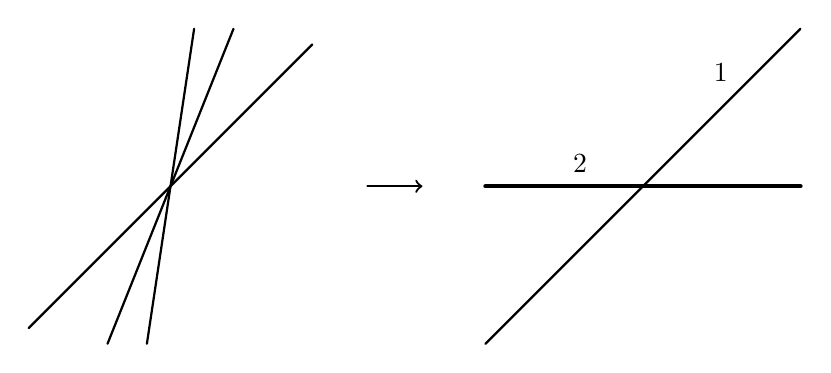
\begin{tikzpicture}[line cap=round, line join=round]

  % --- 左侧图形：三条交汇的直线 ---
  \begin{scope}
    % 最平缓的线
    \draw[thick] (-1.8, -1.8) -- (1.8, 1.8);
    % 中间坡度的线
    \draw[thick] (-0.8, -2)   -- (0.8, 2);
    % 最陡的线
    \draw[thick] (-0.3, -2)   -- (0.3, 2);
  \end{scope}

  % --- 中间的箭头 ---
  \draw[->, thick] (2.5, 0) -- (3.2, 0);

  % --- 右侧图形：水平线和斜线 ---
  \begin{scope}[shift={(6,0)}]
    % 加粗的水平线
    \draw[ultra thick] (-2, 0) -- (2, 0);
    % 斜线
    \draw[thick] (-2, -2) -- (2, 2);

    % 标注数字 2 (在水平线上方)
    \node[above] at (-0.8, 0.05) {2};
    % 标注数字 1 (在斜线上方)
    \node[above left] at (1.2, 1.2) {1};
  \end{scope}

\end{tikzpicture}
\end{center}


对更一般的曲线, 想法相同.

\subsection*{Kodaira 的工作}

在考虑 N\'eron 模型之前, 我们考察一个类似的情形, 即它的先驱. 考虑方程
\[
Y^2Z = X^3 + a(T)XZ^2 + b(T)Z^3, \qquad
\Delta(T) \mathrel{=_{\mathrm{def}}} 4a(T)^3 + 27b(T)^2\neq 0,
\]
其中 $a(T), b(T)\in\mathbb{C}[T]$. 可把它视为定义三个不同对象:
\begin{enumerate}[label=\textup{(\alph*)}]
\item 域 $\mathbb{C}(T)$ 上的椭圆曲线 $E$;
\item $\mathbb{P}^2(\mathbb{C})\times\mathbb{A}^1(\mathbb{C})$ 中的曲面 $S$, 其点是满足方程的序对 $((x:y:z), t)$;
\item 由 $T$ 参数化的 (可能退化的) 椭圆曲线族 $E(T)$.
\end{enumerate}
(c) 的含义如下: 对每个 $t_0\in\mathbb{C}$, 有曲线
\[
E(t_0)\colon Y^2Z = X^3 + a(t_0)XZ^2 + b(t_0)Z^3, \qquad a(t_0), b(t_0)\in\mathbb{C},
\]
带判别式 $\Delta(t_0)$. 当且仅当 $t_0$ 不是多项式 $\Delta(T)$ 的根时它非奇异, 从而是椭圆曲线; 否则它有奇点, 我们把它视为退化椭圆曲线. 注意投影 $\mathbb{P}^2(\mathbb{C})\times\mathbb{A}^1(\mathbb{C})\to\mathbb{A}^1(\mathbb{C})$ 诱导映射 $S\to\mathbb{A}^1(\mathbb{C})$, 其纤维\index{xianwei@纤维(fibre)}正是曲线 $E(t)$. 可把 $S$ 视为 $E$ 在 $\mathbb{C}[T]$ 上 (或 $\mathbb{A}^1(\mathbb{C})$ 上) 的``模型''. 我们应选取 $E$ 的方程使 $\Delta(T)$ 的次数尽可能小, 从而使奇异纤维尽可能少.

为方便, 现在省去 $Z$, 考虑方程
\[
S\colon Y^2 = X^3 + a(T)X + b(T), \qquad a(T), b(T)\in\mathbb{C}[T].
\]
(严格地说, 我们应在射影曲线族上工作.)

设 $P = (x,y,t)\in S(\mathbb{C})$, 令 $f(X,Y,T) = X^3 + a(T)X + b(T) - Y^2$. 则 $P$ 在曲线 $E(t)$ 上奇异当且仅当它满足方程
\[
\frac{\partial f}{\partial Y} = -2Y = 0, \qquad
\frac{\partial f}{\partial X} = 3X^2 + a(T) = 0.
\]
若此外它满足方程
\[
\frac{\partial f}{\partial T} = \frac{da}{dT}X + \frac{db}{dT} = 0,
\]
则它在曲面 $S$ 上奇异. 故 $P$ 可能在纤维 $E(t)$ 中奇异, 而不在 $S$ 上奇异.

\begin{example} \label{thm:2.7.1} 
\begin{enumerate}[label=\textup{(\alph*)}]
\item 考虑方程 $Y^2 = X^3 - T$, $\Delta(T) = 27T^2$. 原点视为曲线 $E(0)\colon Y^2 = X^3$ 上的点时奇异 (事实上是尖点), 但视为曲面 $S\colon Y^2 = X^3 - T$ 上的点时却不奇异. 事实上, $S$ 在原点的切平面是 $(X,Y)$-平面 $T = 0$.
\item 考虑方程 $Y^2 = X^3 - T^2$, $\Delta(T) = 27T^4$. 此时原点视为 $E(0)$ 上的点时奇异, 视为 $S$ 上的点也奇异.
\item 考虑方程
\[
Y^2 = (X - 1 + T)(X - 1 - T)(X + 2) = X^3 - (3 + T^2)X + 2 - 2T^2.
\]
判别式为 $\Delta(T) = -324T^2 + 72T^4 - 4T^6$. 曲线 $E(0)$ 是
\[
Y^2 = X^3 - 3X + 2 = (X-1)^2(X+2),
\]
在 $(1,0)$ 处有结点. 为把 $(1,0,0)$ 平移到原点, 在原方程中用 $X$ 替换 $X - 1$, 方程变为
\[
Y^2 = (X + T)(X - T)(X + 3) = (X^2 - T^2)(X + 3) = X^3 + 3X^2 - T^2X - 3T^2.
\]
此曲面在原点处有奇点, 因为其方程没有线性项.
\end{enumerate}
\end{example}

\cite{kodaira1960} 表明, 通过吹胀 (blowing up) 点、吹缩 (blowing down) 曲线等, 可以从曲面
\[
S\colon Y^2Z = X^3 + a(T)XZ^2 + b(T)Z^3, \qquad a(T), b(T)\in\mathbb{C}[T], \ \Delta(T)\neq 0
\]
得到新曲面 $S_0$ 与正则映射 $S_0\to\mathbb{A}^1$, 具有以下性质:
\begin{enumerate}[label=\textup{(\alph*)}]
\item $S_0$ 非奇异;
\item 把 $S_0$ 视为 $\mathbb{C}(T)$ 上的曲线等于把 $S$ 视为 $\mathbb{C}(T)$ 上的曲线 (对专家: 映射 $S\to\mathbb{A}^1$ 与 $S_0\to\mathbb{A}^1$ 有相同的普通纤维);
\item $S_0$ 在 $\mathbb{A}^1(\mathbb{C})$ 之上的纤维 $E'(t_0)$ 是射影曲线; 且若 $E(t_0)$ 的点视为 $S$ 上的点时非奇异 (例如 $E(t_0)$ 本身非奇异), 则 $E'(t_0) = E(t_0)$;
\item $S_0$ 关于上述性质极小: 若 $S''\to\mathbb{A}^1$ 是具有性质 (a,b,c) 的第二个映射, 则在普通纤维上是同构的每个正则映射 $S_0\to S''$ (在 $\mathbb{A}^1$ 上) 都是同构.
\end{enumerate}
映射 $S_0\to\mathbb{A}^1$ 由这些性质在唯一同构的意义下唯一确定. Kodaira 分类了 $S_0\to\mathbb{A}^1$ 的可能纤维.

``吹胀''曲面 $S$ 的非奇异点 $P$ 保持曲面不变, 只是把点 $P$ 换成 $S$ 在 $P$ 处切平面中过原点的直线射影空间. 对过 $P$ 的曲线 $C$, $C\setminus\{P\}$ 的逆像是吹胀簇中的曲线, 其闭包在射影空间中交于对应 $C$ 在 $P$ 处切线方向的那一点. 即使 $S\subset\mathbb{P}^m$, 吹胀后的曲面也没有自然嵌入射影空间.

\begin{example} \label{thm:2.7.2} 
为说明``吹胀''现象, 考虑映射
\[
\psi\colon k^2\to k^2, \qquad (x,y)\mapsto(x, xy).
\]
它的像只遗漏 $Y$-轴上 $Y\neq 0$ 的点. 像中的点除 $(0,0)$ 外都是 $k^2$ 中唯一点的像, 而 $(0,0)$ 被``吹胀''成整个 $Y$-轴. 换言之, 该映射一对一, 只是 $Y$-轴被``吹缩''成一点. 直线 $L\colon Y = \alpha X$ 的逆像是 $XY = \alpha X$, 它是 $Y$-轴与直线 $Y = \alpha$ 的并; $L\setminus\{(0,0)\}$ 的逆像的闭包是直线 $Y = \alpha$. 奇异曲线
\[
C\colon Y^2 = X^3 + \alpha X^2
\]
的逆像是曲线
\[
Y^2X^2 = X^3 + \alpha X^2,
\]
它是曲线 $X^2 = 0$ (``重数''为 $2$ 的 $Y$-轴) 与非奇异曲线 $Y^2 = X + \alpha$ 的并. 注意后者与 $Y$-轴交于点 $(0,\pm\sqrt{\alpha})$, 即对应 $C$ 在 $(0,0)$ 处切线的斜率的那两点.

此例中, $\mathbb{A}^2(k)$ 中的 $(0,0)$ 被吹胀成一条仿射直线. 在真正的吹胀中, 它将被换成一条射影直线, 且映射的描述更复杂. ($\mathbb{P}^2$ 中点的吹胀见 \cite[Chap. 7]{fulton1969}.)
\end{example}

\subsection*{N\'eron 的工作}

N\'eron 对 $\mathbb{Q}_p$ 上的椭圆曲线证明了 Kodaira 结果的类似物.\footnote{更准确地说, 他证明了 Kodaira 对离散赋值环 $\mathbb{C}[[T]]$ 上曲线得到的结果, 也适用于剩余域完美的任意完备赋值环上的曲线.} 为解释他的结果, 需要谈论概形. 对非专家, $\mathbb{Z}_p$ 上的概形 $\mathcal{E}$ 不过是由系数在 $\mathbb{Z}_p$ 中的多项式方程族定义的对象. 由相同方程 (视为系数在 $\mathbb{Q}_p$ 中) 定义的对象是 $\mathbb{Q}_p$ 上的簇 $E$, 称为 $\mathcal{E}/\mathbb{Z}_p$ 的普通纤维 (generic fibre); 由把系数模 $p$ 的方程定义的对象是 $\mathbb{F}_p$ 上的簇 $\tilde{E}$, 称为 $\mathcal{E}/\mathbb{Z}_p$ 的特殊纤维\index{xianwei@纤维(fibre)!teshu@特殊(special)} (special fibre). 例如, 若 $\mathcal{E}$ 是由方程
\[
Y^2Z + a_1XYZ + a_3YZ^2 = X^3 + a_2X^2Z + a_4XZ^2 + a_6Z^3, \qquad a_i\in\mathbb{Z}_p
\]
定义的概形, 则 $E$ 是由相同方程定义的 $\mathbb{Q}_p$ 上椭圆曲线, $\tilde{E}$ 是由方程
\[
Y^2Z + \tilde{a}_1XYZ + \tilde{a}_3YZ^2 = X^3 + \tilde{a}_2X^2Z + \tilde{a}_4XZ^2 + \tilde{a}_6Z^3
\]
定义的 $\mathbb{F}_p$ 上椭圆曲线, 其中 $\tilde{a}_i$ 是 $a_i$ 在 $\mathbb{Z}/p\mathbb{Z} = \mathbb{F}_p$ 中的像.

给定椭圆曲线 $E/\mathbb{Q}_p$, N\'eron 构造具有如下性质的 $\mathbb{Z}_p$ 上概形 $\mathcal{E}$:
\begin{enumerate}[label=\textup{(\alph*)}]
\item $\mathcal{E}$ 正则 (regular), 即所有相伴局部环都是正则局部环 (若局部环维数为 $d$, 则其极大理想可由 $d$ 个元素生成). (对代数闭域上的代数簇, ``正则''等价于``非奇异''.)
\item $\mathcal{E}$ 的普通纤维是原来的曲线 $E$;
\item $\mathcal{E}$ 在 $\mathbb{Z}_p$ 上真 (proper), 即 $\tilde{E}$ 是射影曲线;
\item $\mathcal{E}$ 关于上述性质极小: 若 $\mathcal{E}'$ 是 $\mathbb{Z}_p$ 上具有性质 (a,b,c) 的第二个概形, 则在普通纤维上是同构的每个 $\mathbb{Z}_p$ 上正则映射 $\mathcal{E}\to\mathcal{E}'$ 都是同构.
\end{enumerate}
且 N\'eron 分类了 $\mathbb{F}_p^{\mathrm{al}}$ 上可能的特殊纤维, 得到与 Kodaira 本质上相同的列表.

$\mathbb{Z}_p$ 上的曲线 $\mathcal{E}$ 称为完全 N\'eron (极小) 模型.\index{moxing@模型(model)!wanquan-Neron@完全 N\'eron(complete Néron model)} 它有些缺点: 未必有 $\mathcal{E}(\mathbb{Z}_p)\cong E(\mathbb{Q}_p)$; 它没有群结构; 其特殊纤维 $\tilde{E}$ 可能奇异. 三个缺点都可通过简单地去掉特殊纤维中的全部奇点与多重曲线来消除. 由此得到光滑 N\'eron (极小) 模型\index{moxing@模型(model)!guanghua-Neron@光滑 N\'eron(smooth Néron model)}, 但它的缺点是不再真.

给定 $\mathbb{Q}_p$ 上的椭圆曲线 $E$, 我们现在在 $\mathbb{Z}_p$ 上有三个模型:
\begin{enumerate}[label=\textup{(\alph*)}]
\item $\mathcal{E}_w$, $E$ 的 Weierstrass 极小模型;
\item $\mathcal{E}$, $E$ 的完全 N\'eron 模型;
\item $\mathcal{E}^0$, $E$ 的光滑 N\'eron 模型.
\end{enumerate}
它们的关系如下: 从 $\mathcal{E}$ 得到 $\mathcal{E}^0$, 需去掉全部多重曲线与奇点; 从 $\mathcal{E}^0$ 得到去掉闭纤维中奇异点的 Weierstrass 模型, 需去掉特殊纤维中除含 $O$ 的分支外的所有连通分支.

\begin{aside} \label{thm:2.7.3} 
按定义, 阿贝尔簇 (abelian variety)\index{abeiercu@阿贝尔簇(abelian variety)} 是带有正则映射定义的群结构的射影代数簇. 故一维阿贝尔簇即椭圆曲线. 椭圆曲线理论的许多 (但非全部) 内容可推广到所有阿贝尔簇, 但因不再能写出方程, 证明需要多得多的代数几何机器. 对维数 $> 1$ 的阿贝尔簇, 只有光滑 N\'eron 极小模型存在.
\end{aside}

\subsection*{不同类型}

我们描述十种 (或按计数方式不同为十一种) 可能模型类型中的三种, 同时使用 Kodaira 编号 ($I_0, I_n, II, \dots$) 与 N\'eron 编号 ($a, b_n, c_1, \dots$). 我们描述 $\mathbb{F}_p$ 的代数闭包而非 $\mathbb{F}_p$ 本身上的特殊纤维. 例如, 在结点约化 (型 $(I_n, b_n)$) 情形, 光滑 N\'eron 模型的特殊纤维的单位连通分支将是 $\mathbb{F}_p$ 上扭的 $\mathbb{G}_m$, 除非切线有理, 且特殊纤维的某些分支在 $\mathbb{F}_p$ 上可能不有理.

\subsection*{($I_0$, a)} 此时 $E$ 有好约化, 三个模型都相同.

\paragraph*{($I_n$, $b_n$), $n>1$} 此时 $E$ 有结点约化; 设 $n = \ord\nolimits_p(\Delta)$; 三个模型的特殊纤维如下:
\begin{enumerate}[label=\textup{(\alph*)}]
\item 带结点的三次曲线;
\item $n$ 条亏格 $0$ 的曲线, 每条恰与另外两条相交;
\item 代数群 $G$, 其单位连通分支 $G^\circ$ 是 $\mathbb{G}_m$, 且 $G/G^\circ$ 是 $n$ 阶循环群.
\end{enumerate}

\begin{center}
\begin{tikzpicture}[line cap=round, line join=round, thick]

  % --- 图 (a): 节点三次曲线 (Nodal Cubic) ---
  \begin{scope}[shift={(0,0)}]
    % 使用参数方程绘制曲线: x = 1 - t^2, y = t(1 - t^2)
    % 调整系数以匹配原图比例
    \draw plot[domain=-1.4:1.4, samples=100] ({-1.5*(\x*\x-1)}, {1.5*\x*(\x*\x-1)});
    \node at (0, -2.5) {(a)};
  \end{scope}

  % --- 图 (b): 带延长线交点的六边形 ---
  \begin{scope}[shift={(5,0)}]
    % 定义六边形的顶点坐标
    \foreach \a [count=\i] in {60, 120, 180, 240, 300, 360} {
      \coordinate (V\i) at (\a:1.3);
    }
    
    % 绘制边，并向两端延长以产生交点效果
    % 这里的 \shorten 是负值，表示向外延长
    \draw[shorten <=-0.3cm, shorten >=-0.3cm] (V1) -- (V2);
    \draw[shorten <=-0.3cm, shorten >=-0.3cm] (V2) -- (V3);
    \draw[shorten <=-0.3cm, shorten >=-0.3cm] (V3) -- (V4);
    \draw[shorten <=-0.3cm, shorten >=-0.3cm] (V4) -- (V5);
    \draw[shorten <=-0.3cm, shorten >=-0.3cm] (V6) -- (V1);
    
    % 图中右下角的边是虚线 (dotted)
    \draw[dotted, shorten <=-0.1cm, shorten >=-0.1cm] (V5) -- (V6);

    \node at (0, -2.5) {(b)};
  \end{scope}

  % --- 图 (c): 文字描述 ---
  \begin{scope}[shift={(9.5,0)}]
    \node[align=center, text width=3cm] at (0,0) {
      相同, 但是没有交点.
    };
    \node at (0, -2.5) {(c)};
  \end{scope}

\end{tikzpicture}
\end{center}

\paragraph*{($I_0^*$, $c_4$)} 此时 $E$ 有尖点约化且 $\ord\nolimits_p(\Delta) = 6$ ($p\neq 2$); 三个模型的特殊纤维如下:
\begin{enumerate}[label=\textup{(\alph*)}]
\item 带尖点的三次曲线;
\item 四条不相交的、重数 $1$ 的亏格 $0$ 曲线, 连同一条重数 $2$、横截穿过四条曲线中每一条的亏格 $0$ 曲线;
\item 代数群 $G$, 其单位连通分支是 $\mathbb{G}_a$, 且 $G/G^\circ$ 是同构于 $\mathbb{Z}/2\mathbb{Z}\times\mathbb{Z}/2\mathbb{Z}$ 的 $4$ 阶群.
\end{enumerate}

\begin{center}
\begin{tikzpicture}[line cap=round, line join=round, thick]

  % --- 图 (a): 尖点曲线 (Cusp Curve) ---
  % 使用参数方程 x = -t^2, y = t^3 来绘制典型的尖点形状
  \begin{scope}[shift={(0,0)}]
    \draw plot[domain=-1.4:1.4, samples=100] ({1.5 - \x*\x}, {0.7*\x*\x*\x});
    \node at (0.5, -2.5) {(a)};
  \end{scope}

  % --- 图 (b): 带有数字标注的相交直线 ---
  \begin{scope}[shift={(5,0)}]
    % 垂直主线
    \draw (0, -1.8) -- (0, 1.8);
    
    % 上方的两条平行斜线 (向下倾斜)
    \draw (-0.8, 1.8) -- (1, 0.8);
    \draw (-0.8, 1.3) -- (1, 0.3);
    
    % 下方的两条平行斜线 (向上倾斜)
    \draw (-0.8, -1.8) -- (1, -0.8);
    \draw (-0.8, -1.3) -- (1, -0.3);
    
    % 数字标注
    \node[above] at (-0.2, 1.4) {1};
    \node[above] at (-0.2, 0.9) {1};
    \node[left]  at (0, 0)   {2};
    \node[above] at (-0.2, -0.8) {1};
    \node[above] at (-0.2, -1.4) {1};

    \node at (0.1, -2.5) {(b)};
  \end{scope}

  % --- 图 (c): 多行文字说明 ---
  \begin{scope}[shift={(9.5,0)}]
    \node[align=center, text width=3.5cm] at (0,0) {
      相同, 但没有多重曲线包括其交点.
    };
    \node at (0, -2.5) {(c)};
  \end{scope}

\end{tikzpicture}
\end{center}

(从 (a) 到 (b) 需去掉重曲线包括其交点; 从 (b) 到 (c) 再去掉.)

使用极小方程时, \S\ref{sec:2.4} 中神秘的商 $E(\mathbb{Q}_p)/E^0(\mathbb{Q}_p)$ 等于 $G(\mathbb{F}_p)/G^\circ(\mathbb{F}_p)$, 其中 $G$ 是光滑 N\'eron 模型的特殊纤维, $G^\circ$ 是 $G$ 的单位连通分支. 在上述三个例子中, 它分别是 (a) 平凡群; (b) $n$ 阶循环群的子群 (若 $E$ 有分裂结点约化则等于 $n$ 阶循环群); (c) $(\mathbb{Z}/2\mathbb{Z})^2$ 的子群.

\subsection*{极小模型的总结}

\begin{center}
\renewcommand{\arraystretch}{1.3}
\begin{tabular}{lccc}
\hline
& Weierstrass & 完全 N\'eron & 光滑 N\'eron\\
\hline
$E$ 是平面曲线 & 是 & 不一定 & 不一定\\
$E$ 正则 & 不一定 & 是 & 是\\
$\tilde{E}$ 射影 & 是 & 是 & 不一定\\
$\tilde{E}$ 非奇异 & 不一定 & 不一定 & 是\\
$\tilde{E}$ 是群 & 不一定 & 不一定 & 是\\
\hline
\end{tabular}
\end{center}

\section{椭圆曲线的算法}\label{sec:2.8}

1965 年前后, Weil 提出 $\mathbb{Q}$ 上固定导子 $N$ 的椭圆曲线与 $\Gamma_0(N)$ 的 $-2$ 维尖点形式之间存在精确对应 (\cite{weil1967}; 见 V, \S\ref{sec:5.5}). 这促使 Tate\footnote{``同一年 (65--66 年), 我从巴黎给 Cassels 写信. 我记得那是在秋天. 那年夏初, Weil 告诉了我所有 $\mathbb{Q}$ 上椭圆曲线都是模曲线的想法. 这激励 Swinnerton-Dyer 对判别式不太大的 $\mathbb{Q}$ 上椭圆曲线做大型计算机搜索, 以检验 Weil 的想法. 但当然必须能计算导子才能做那个检验. 那是我主要的动机. 我不知道为什么我写信给 Cassels 而不是 Swinnerton-Dyer. 也许因为我更了解他.'' Tate, 私人通信.} 找出计算 $\mathbb{Q}$ 上椭圆曲线极小 Weierstrass 方程、判别式、导子、$j$-不变量、N\'eron 模型纤维等的算法, 以便检验 Weil 的想法. 他把它们写进前面提到的给 Cassels 的信中, 即后来发表的 \cite{tate1975}. 这些算法对人类来说痛苦, 但对计算机容易. 幸运的是, 它们已在计算机程序中实现, 例如专门为代数数论 (包括椭圆曲线) 计算设计的 Pari/gp 程序. 下面我解释如何把 Pari 当作超级计算器使用. 也可以编程, 但那需要读手册.

回忆域 $k$ 上椭圆曲线 $E$ 的一般 Weierstrass 方程~\eqref{eq:11} 为
\[
Y^2Z + a_1XYZ + a_3YZ^2 = X^3 + a_2X^2Z + a_4XZ^2 + a_6Z^3,
\]
且依附于曲线量 $b_2, b_4, b_6, b_8, c_4, c_6$ 与
\[
\Delta = -b_2^2b_8 - 8b_4^3 - 27b_6^2 + 9b_2b_4b_6, \qquad j = c_4^3/\Delta.
\]
曲线非奇异当且仅当 $\Delta\neq 0$. 微分形式 $\omega = \frac{dx}{2y + a_1x + a_3}$ 在平移下不变. 椭圆曲线 $E$ 的 Weierstrass 方程在如下坐标变换下确定到唯一:
\[
X = u^2X' + r, \qquad Y = u^3Y' + su^2X' + t, \qquad u,r,s,t\in k, \ u\neq 0.
\]
量 $\Delta$, $j$, $\omega$ 按如下规则变换:
\[
u^{12}\Delta' = \Delta, \qquad j' = j, \qquad \omega' = u\omega.
\]
$\mathbb{Q}$ 上椭圆曲线 $E$ 的极小 Weierstrass 方程是上述形式的、$a_i\in\mathbb{Z}$ 且 $\Delta$ 极小的方程. 它在带 $r,s,t,u\in\mathbb{Z}$, $u\in\mathbb{Z}^{\times} = \{\pm 1\}$ 的上述坐标变换下确定到唯一.

在 gp (grande calculatrice pari) 中, 椭圆曲线由向量
\[
v = [a_1, a_2, a_3, a_4, a_6]
\]
指定.

\begin{center}
\renewcommand{\arraystretch}{1.35}
\begin{tabular}{@{}p{0.38\linewidth}p{\dimexpr0.62\linewidth-2\tabcolsep\relax}@{}}
\texttt{e=ellinit(v,1)} & 把 $e$ 定义为椭圆曲线 $Y^2 + a_1XYZ + \cdots$, 并计算 13 分量向量\\
& $[a_1,\allowbreak a_2,\allowbreak a_3,\allowbreak a_4,\allowbreak a_6,\allowbreak b_2,\allowbreak b_4,\allowbreak b_6,\allowbreak b_8,\allowbreak c_4,\allowbreak c_6,\allowbreak \Delta,\allowbreak j]$\\
\texttt{e=ellinit(v)} & 把 $e$ 定义为椭圆曲线 $Y^2 + a_1XYZ + \cdots$, 并计算上述 13 分量向量\\
& 连同一些对其他计算有用的额外信息\\
\texttt{elladd(e,z1,z2)} & 计算 $e$ 上点 $z_1 = [x_1, y_2]$ 与 $z_2 = [x_2, y_2]$ 的和\\
\texttt{elltors(e)} & 计算 $[t, v_1, v_2]$, 其中 $t$ 是 $E(\mathbb{Q})_{\mathrm{tors}}$ 的阶, $v_1$ 给出\\
& $E(\mathbb{Q})_{\mathrm{tors}}$ 作为循环群乘积的结构, $v_2$ 给出循环群的生成元\\
\texttt{ellglobalred(e)} & 计算向量 $[N, v, c]$, 其中 $N$ 是曲线的导子, $v = [u, r, s, t]$\\
& 是化为 Weierstrass 极小模型的坐标变换 (其中 $a_1 = 0$ 或 $1$, $a_2 = 0, 1, -1$,\\
& $a_3 = 0, 1$). 这样的模型唯一\\
\texttt{e0=ellchangecurve(e,v)} & 把 $e$ 换成 $e_0$, 其中 $e_0$ 是对应于由坐标变换\\
& $v = [u, r, s, t]$ 得到的曲线的 $13{+}$ 分量向量\\
\texttt{ellocalred(e,p)} & 用 Kodaira 记号计算在 $p$ 处约化的类型. 产生 $[f, n, \dots]$,\\
& 其中 $f$ 是 $p$ 在 $e$ 的导子中的指数, $n = 1$ 表示好约化 (型 $I_0$),\\
& $n = 2, 3, 4$ 表示型 $II, III, IV$ 的约化, $n = 4+\nu$ 表示型 $I_\nu$,\\
& $-1, -2$ 等表示 $I_0^*, II^*, \dots$\\
\texttt{ellap(e,p)} & 计算 $a_p \mathrel{=_{\mathrm{def}}} p + 1 - \#E(\mathbb{F}_p)$. 要求 $e$ 在 $p$ 处极小\\
\texttt{ellan(e,n)} & 计算前 $n$ 个 $a_k$. 要求 $e$ 在 $p$ 处极小\\
\texttt{ellgenerators(e)} & 计算 $E(\mathbb{Q})/\mathrm{tors}$ 的基 (要求 John Cremona 的椭圆曲线数据可用)
\end{tabular}
\end{center}

\subsection*{例子 (Example)}

启动 gp.
\begin{verbatim}
gp>  v=[0,-4,0,0,16]
\end{verbatim}
把 $v$ 设为向量 $(0,-4,\dots)$.
\begin{verbatim}
%1 = [0,-4,0,0,16]
gp>  ellinit(v,1)
\end{verbatim}
计算向量 $(a_1,\dots,j)$.
\begin{verbatim}
%2 = [0,-4,0,0,16,-16,0,64,-256,256,-9728,-45056,-4096/11]
\end{verbatim}
例如, $\Delta = -45056$, $j = -4096/11$.
\begin{verbatim}
gp>  e=ellinit(v)
\end{verbatim}
计算向量 $(a_1,\dots,j,\dots)$, 并把 $e$ 设为椭圆曲线 $Y^2 = X^3 - 4X^2 + 16$.
\begin{verbatim}
%3 = [0,-4,0,0,16,...]
gp>  elltors(e)
\end{verbatim}
计算挠子群 (它是 $5$ 阶循环群).
\begin{verbatim}
%4 = [5,[5],[0,4]]
gp>  ellglobalred(e)
\end{verbatim}
计算最小导子与给出极小方程所需的坐标变换.
\begin{verbatim}
%5 = [11, [2,0,0,4], 1]
gp>  ellchangecurve(e,[2,0,0,4])
%6 = [0,-1,1,0,0,-4,0,1,-1,16,-152,-11,-4096/11,...]
\end{verbatim}
计算 $E$ 的极小方程 $Y^2 + Y = X^3 - X^2$, 它现在有判别式 $-11$, 但 (当然) 相同的 $j$-不变量.
\begin{verbatim}
gp>  elllocalred(%6,2)
%7 = [0,1,[1,0,0,0],1]
\end{verbatim}
所以 $E$ 现在在 $2$ 处有好约化.
\begin{verbatim}
gp>  elllocalred(%6,11)
%8 = [1,5,[1,0,0,0],1]
\end{verbatim}
所以 $E$ 在 $11$ 处有坏约化, 导子为 $11^1$ (故奇点是结点), 且 N\'eron 模型特殊纤维的 Kodaira 型是 $I_1$.
\begin{verbatim}
gp>  ellap(%6,13)
\end{verbatim}
计算 $a_{13}$.
\begin{verbatim}
%9 = 4
\end{verbatim}
所以 $\#E(\mathbb{F}_{13}) = 13 + 1 - 4 = 10$.
\begin{verbatim}
gp>  ellgenerators(e)
%10 = []
\end{verbatim}
所以 $E(\mathbb{Q})$ 有限.
\begin{verbatim}
gp>  ellinit([6,-3,9,-16,-14])
%11 = [6,-3,9,-16,-14,24,22,25,29,48,-216,37,110592/37,...]
gp>  ellgenerators(%11)
%12 = [[-2,2]]
\end{verbatim}
所以 $E(\mathbb{Q})/\mathrm{tors}$ 是由 $(-2,2)$ 生成的秩 $1$ 自由模.

{\emergencystretch=3em Pari/gp 可从 \url{https://pari.math.u-bordeaux.fr/} 免费获取. 推荐以下资料: 书 \cite{cohen1993}、\cite{cohen2000} 与 \cite{cremona1997}; 数据库 \textit{The L-functions and Modular Forms Database} (\url{https://www.lmfdb.org/}); 文章 \cite{best2020}.\par}
